\documentclass[11pt,a4paper,twoside]{book}
\includeonly{ch4_anomalien/anomalien}
\usepackage{ngerman}
\usepackage{graphicx}
\usepackage{epsfig}
\usepackage{epstopdf}
\usepackage[onehalfspacing]{setspace}
\usepackage[hidelinks]{hyperref}
\usepackage{tocloft}
\usepackage{tikz}
\usetikzlibrary{matrix}
\usepackage{float}
\usepackage{amsmath}
\usepackage{amssymb}
\usepackage{subcaption}
\usepackage{colortbl}
\usepackage{xcolor}
\usepackage{slashbox}
\usepackage{array}
\usepackage{multirow}

% Seitenlayout anpassen
% \setlength{\textheight}{25cm}
% \setlength{\textwidth}{17cm}
% \setlength{\topmargin}{-15mm}
% \setlength{\parindent}{0ex}
% \setlength{\parskip}{2ex}
% \setlength{\oddsidemargin}{-6.5mm}
% \setlength{\evensidemargin}{-16.5mm}
\usepackage[a4paper,
            top=25mm,      % Abstand oben
            bottom=25mm,   % Abstand unten
            inner=25mm,    % Innenrand (für Bindung)
            outer=15mm,    % Außenrand (für Symmetrie)
            heightrounded, % Höhe wird gerundet
            includehead,   % Kopfzeile wird in Layout eingeschlossen
            includefoot    % Fußzeile wird in Layout eingeschlossen
           ]{geometry}
\setlength{\parindent}{0ex} % Kein Einzug am Absatzbeginn
\setlength{\parskip}{2ex}   % Abstand zwischen Absätzen

% Inhaltsverzeichnis anpassen
\renewcommand{\cftchapfont}{\bfseries} % Kapitel fett
\renewcommand{\cftsecfont}{}           % Sektionen nicht fett
\renewcommand{\cftdotsep}{2}           % Punkte zwischen Titel und Seitenzahl

% Literaturverzeichnis alphabetisch und mit anderem Titel
\usepackage[backend=biber,style=numeric,sorting=nyt]{biblatex}
\addbibresource{Thesis_BIB.bib}
\AtBeginDocument{
  \renewcommand{\bibname}{Literaturverzeichnis}
}

\begin{document}

% Deckblatt und Verzeichnisse
%%%%%%%%%%%%%%%%%%%%%%%%%%%%%%%%%%%%%%%%%%%%
% deckblatt-BT-ET-IT-ger-v20170301.tex
% Deckblatt 
% Bachelorstudiengang Elektrotechnik
% Studienrichtung Elektrotechnik & Informationstechnik
%
% author:        		K.H. Hofmann 
% created:       	07.08.2014
% last revision:	01.03.2017
%%%%%%%%%%%%%%%%%%%%%%%%%%%%%%%%%%%%%%%%%%%%

% Page border should be:
% top: 15 mm
% oddside:  left 25 mm, right 15 mm
% evenside: left 15 mm, right 25 mm
%
% Eingaben
\newcommand{\Bearbeiter}{Moritz Mühlhausen}
\newcommand{\Thema}{Anomaliedetektion zur Entwicklung eines Predictive Maintenance Systems in der Verkehrstechnik}
%%%%%%%%%%%%%%%%%%%%%%%%%%%%%%%%%%%%%%%%%%%%
%\begin{document}
%%%%%%%%%%%%%%%%%%%%%%%%%%%%%%%%%%%%%%%%%%%%
% Deckblatt 1. Seite 
\thispagestyle{empty} 
%
\vspace{-20mm}
\begin{minipage}[t]{8cm}  

\epsfig{file=deckblatt/Logo-HsRm-1.eps,width=6cm}
\end{minipage}
\hfill
\raisebox{4.3ex}{\small \begin{tabular}[t]{l}
{\textbf{Fachbereich}} \\
Ingenieurwissenschaften \\[1ex]
{\textbf{Studienbereich}} \\
Informationstechnologie und Elektrotechnik \\[1ex]
{\textbf{Studiengang}} \\ 
Elektrotechnik \\[1ex]
{\textbf{Studienrichtung}} \\ 
Elektrotechnik \& Informationstechnik 
\end{tabular}}
\vspace{30mm}
\begin{center}{\Huge\bf Bachelor Thesis} \par
\vspace{20mm}
{\LARGE\bf  \Thema} \par
\vspace{16mm}
{\LARGE\bf  \Bearbeiter} \par
\end{center}
% 
\vspace{15mm}
\begin{flushright}
    Vorgelegt am (Stempel des Studienbereichs): \\
    \vspace{20mm} % Wenn mehr Platz nötig ist
    \rule[0ex]{\textwidth}{0.4pt} \hspace{5mm} (Ort / Datum) \hspace{30ex} (Unterschrift Student)
\end{flushright}
\vfill
\begin{flushleft}
\begin{tabular}{ll}
    Referent:	 &  Prof.\ Dr.-Ing. Michael Voigt \\ [0.5ex]
    Korreferent:	 &  M. Sc. Felix Becker, Vitronic Machine Vision GmbH
\end{tabular}
\end{flushleft}
%%%%%%%%%%%%%%%%%%%%%%%%%%%%%%%%%%%%%%%%%%%%
% Blankoseite
\newpage
\thispagestyle{empty}
\rule[0ex]{0ex}{0ex} 	% unsichtbare Markierung, damit Leerseite möglich
%%%%%%%%%%%%%%%%%%%%%%%%%%%%%%%%%%%%%%%%%%%%
% Versicherung
\newpage
\thispagestyle{empty} 
%
{\bf Versicherung}
\par
Hiermit versichere ich, dass ich die vorliegende Arbeit selbst\"andig und ohne unzul\"assige Hilfe Dritter verfasst 
habe.
\par
Die aus fremden Quellen direkt oder indirekt \"ubernommenen Texte, Gedankeng\"ange, Konzepte usw.\ in meinen 
Ausf\"uhrungen habe ich als solche eindeutig gekennzeichnet und mit vollst\"andigen Verweisen auf die jeweilige 
Urheberschaft und Quelle versehen.
\par
Alle weiteren Inhalte wie Textteile, Abbildungen, Tabellen etc.\ ohne entsprechende Verweise stammen im 
urheberrechtlichen Sinn von mir.
\par
Die vorliegende Arbeit wurde bisher weder im In- noch im Ausland in gleicher oder \"ahnlicher Form einer anderen 
Pr\"ufungsbeh\"orde vorgelegt.
\par
Mir ist bekannt, dass ein T\"auschungsversuch vorliegt, wenn sich eine der vorstehenden Versicherungen als 
unrichtig erweist.
\par
\vspace{25mm}
\rule[0ex]{\textwidth}{0.4pt}
(Ort / Datum)\hspace{30ex}	(Unterschrift Student)
%%%%%%%%%%%%%%%%%%%%%%%%%%%%%%%%%%%%%%%%%%%%
% Erklärung zur Einsicht in die Arbeit
\newpage
\thispagestyle{empty} 
%
Der Einsicht in die Bachelor Thesis  und der Ausleihe eines Exemplars der Thesis stimme ich zu / stimme ich nicht zu*.
\par\vspace{10mm}
\rule[0ex]{\textwidth}{0.4pt}
(Ort / Datum)\hspace{30ex}	(Unterschrift Studentin/Student)
\par\vspace{10mm}
Die Zustimmung kann nur bei Vorliegen eines berechtigten Interesses (z.B.\ laufende Forschungsprojekte / Patentschutz) 
verweigert werden. 
\par
Begr\"undung (bei Verweigerung): \\[5ex]
\rule[0ex]{\textwidth}{0.4pt} \\[2ex]
\rule[0ex]{\textwidth}{0.4pt} \\[2ex]
\rule[0ex]{\textwidth}{0.4pt} \\[2ex]
\rule[0ex]{\textwidth}{0.4pt} \\[2ex]
\rule[0ex]{\textwidth}{0.4pt} \\[5ex]
Nur vom Betreuer auszuf\"ullen: \\[2ex]
Gegen die Einsicht in die Bachelor Thesis  und gegen die Ausleihe eines Exemplars der Thesis wird / kein* Einspruch 
erhoben.
\par \vspace{10mm}
\rule[0ex]{\textwidth}{0.4pt}\\
(Ort / Datum)\hspace{30ex} (Unterschrift Betreuer)
\par
Begr\"undung (bei Einspruch): \\[5ex]
\rule[0ex]{\textwidth}{0.4pt} \\[2ex]
\rule[0ex]{\textwidth}{0.0pt} \\[2ex]
\rule[0ex]{\textwidth}{0.4pt} \\[2ex]
\rule[0ex]{\textwidth}{0.4pt} \\[5ex]
*Nichtzutreffendes bitte streichen
%%%%%%%%%%%%%%%%%%%%%%%%%%%%%%%%%%%%%%%%%%%%
%\end{document}
%%%%%%%%%%%%%%%%%%%%%%%%%%%%%%%%%%%%%%%%%%%%

\pagenumbering{arabic}
\chapter{Einleitung und Motivation}
Vitronic Mautbrücken sind aufgrund ihrer schweren Erreichbarkeit und der Tatsache, dass sie über Autobahnen installiert
sind, eine besondere Herausforderung im Bereich der Wartung. Jede Inspektion oder Reparatur erfordert nicht nur die
Bereitstellung spezialisierter Techniker und Geräte, sondern auch eine präzise Planung, um Verkehrsstörungen zu
minimieren und die Sicherheit sowohl der Wartungsteams als auch der Verkehrsteilnehmer zu gewährleisten.

Ein technischer Defekt erfordert häufig eine komplexe Koordination mehrerer Teams und führt zu Verkehrsstörungen. Dadurch
entsteht die Notwendigkeit, Wartungseinsätze effizienter zu gestalten, um die Funktionalität der Infrastruktur und die
Sicherheit der Verkehrsteilnehmenden sowie der Servicemitarbeitenden zu gewährleisten. Gleichzeitig wächst der Druck, diese
Einsätze planbarer und seltener durchzuführen. Genau hier setzt die Motivation dieser Arbeit an: neue Methoden zu entwickeln, die
eine präzise Überwachung des Zustands der Brücken ermöglichen, ohne ständige physische Präsenz vor Ort.

Diese Arbeit befasst sich konkret mit der \textbf{Smart Sensor Platform X1}~-~kurz \textbf{SSPX1}, einem System zur
Erfassung, Verarbeitung und Weiterleitung von Bilddaten. Die vorhandenen Komponenten zur Mautüberwachung umfassen zwei Kameras,
ein eingebettetes High-Performance-Computermodul mit GPU-Unterstützung, ein High-Power-LED-Blitzmodul sowie
eine Stromversorgungshardware mit Weitbereichsspannungseingang. Die SSPX1 nutzt zahlreiche Sensordaten zur
kontinuierlichen und sorgfältigen Überwachung des Systemzustands.

\textbf{Predictive Maintenance} nutzt diese Daten, um Ausfälle vorherzusagen. Sie basiert auf der Analyse
von Echtzeitdaten, die aus einer Vielzahl von Sensoren entnommen werden können. Maschinelles Lernen bietet sich hier als effektive
Methode an, um sich anbahnende Fehler und Ausfälle vorherzusagen und abzufangen. So können Ressourcen effizient
genutzt und Ausfallzeiten minimiert werden~\cite{TobonMejia2012}.

Diese großen Datensätze werden über einen OPC UA Server zur Verfügung gestellt. OPC UA steht für \textit{Open Platform Communication
Unified Architecture} und ist ein Industriestandard für Datenaustausch sowie horizontale und vertikale Kommunikation, unter Anderem
aufgrund seiner Herstellerunabhängigkeit~\cite{Babel2024}.
Die Datenerfassung erfolgt lokal auf jeder SSPX1, welche im Zuge dessen auch einen eigenen Server betreibt, um die aufgenommenen
Daten bereitzustellen. Auf diese Weise wird eine dezentrale Sammlung relevanter Parameter wie Temperatur,
Leistung und Systemauslastung ermöglicht. Die kontinuierliche Überwachung und Speicherung dieser Daten in einer Datenbank
bildet die Grundlage für die Entwicklung und Anwendung prädiktiver Wartungsstrategien.

Ein zentraler Aspekt dabei ist die Detektion von Anomalien, die als Abweichungen vom normalen Verhalten definiert
werden~\cite{Chandola2009}. In multivariaten Systemen erschwert die hohe Dimensionalität und Komplexität der Daten ihre Erkennung.
Unüberwachte maschinelle Lernverfahren bzw.~\textbf{Unsupervised Learning} erweisen sich hier als besonders vielversprechend,
da sie Muster und Zusammenhänge in hochdimensionalen, unstrukturierten Datensätzen identifizieren können, ohne auf eine vorherige
Datenkennzeichnung angewiesen zu sein~\cite{Chandola2009, Wenig2024}.

Ziel dieser Arbeit ist es, Unsupervised Learning Algorithmen für die Erkennung und Interpretation von Anomalien in
heterogenen Datensätzen eines Systems in der Verkehrstechnik zu nutzen und damit die Effizienz von Predictive Maintenance
in der Verkehrstechnik zu optimieren. Dies soll durch eine frühzeitige Identifikation potenzieller Fehler erreicht werden.

Dabei wird zunächst in~\hyperref[ch:pdm_theorie]{Kap.~\ref*{ch:pdm_theorie}} ein theoretischer Hintergrund über die Grundlagen
von Predictive Maintenance und verschiedener Machine Learning Ansätze gegeben und warum sich Unsupervised Learning optimal für
die hier genannten Zwecke eignet.
% weitere Kapitel vorstellen ...

\newpage
\chapter{Zielsetzung}\label{ch:zielsetzung}
Eine effiziente Ressourcennutzung ist für Unternehmen von zentraler Bedeutung. Produktionsprobleme können dabei enorme finanzielle
Verluste verursachen, wie das Beispiel von Volkswagen im Jahr 2016 zeigt: Durch Störungen im Fertigungsprozess entstand ein wöchentlicher
Schaden von bis zu 400 Millionen Euro~\cite{Krupitzer2020}. Zudem zeigen Studien, dass je nach Branche zwischen 15 und 70~\% der
Produktionskosten auf wartungstechnische Ursachen zurückzuführen sind~\cite{Bevilacqua2000}.

Jedoch liegt der Fokus dieser Arbeit nicht auf wirtschaftlichen Faktoren. Trotzdem ist zu erwähnen, dass neue, effiziente
Wartungsstrategien basierend auf der Überwachung wichtiger Systemparameter insgesamt eine wirtschaftlichere und kostengünstigere
Alternative zu klassischen Wartungsstrategien (vgl.~\hyperref[sec:trad_maintenance]{Abs.~\Ref*{sec:trad_maintenance}})
darstellen~\cite{Deloux2009}~\Cite[S.~64--65]{Mobley2002}.

Der Fokus liegt vielmehr in der Entwicklung, Erprobung und Umsetzung der zugrundeliegenden technischen Fragestellung: \textbf{Wie können
Algorithmen zur Anomaliedetektion genutzt werden, um zur Entwicklung eines effizienten Wartungssystems
beizutragen?}

\begin{figure}[b!]
    \centering
    \begin{tikzpicture}
        \node[anchor=south west,inner sep=0] (image) at (0,0) {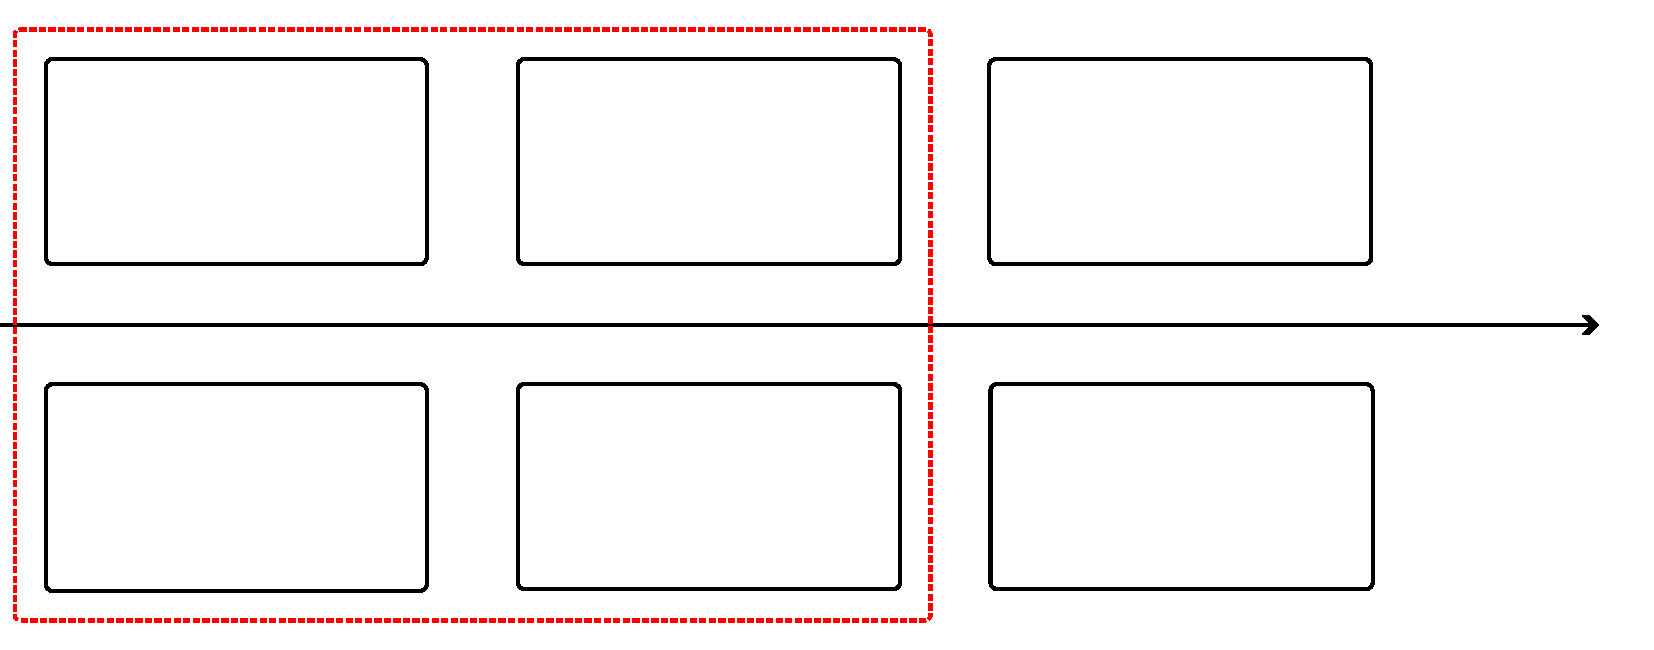
\includegraphics[width=1\linewidth]{ch2_zielsetzung/abbildungen/zielsetzung_scope.pdf}};
        % Koordinatensystem für die Grafik
        \begin{scope}[x={(image.south east)},y={(image.north west)}]
            % Textpositionen anpassen:
            \node at (0.145,0.74) {\large\parbox{6cm}{\centering Daten-\\aggregierung}};
            \node at (0.145,0.26) {\large\parbox{6cm}{\centering Recherche\\sich eignender\\Algorithmen}};
            \node at (0.43,0.74) {\large\parbox{4cm}{\centering Implementierung \&\\Erprobung der\\Algorithmen}};
            \node at (0.43,0.26) {\large\centering Evaluierung};
            \node at (0.715,0.74) {\large\parbox{4cm}{\centering Ableitung\\geeigneter\\Maßnahmen}};
            \node at (0.715,0.26) {\large\parbox{4cm}{\centering Schulen und Finden\\geeigneter\\Mitarbeiter}};
            \node at (0.85,0.46) {\centering Entwicklungsfortschritt};
            \node at (0.2875,0) {\centering \textcolor{red}{\large\textbf{Fokus der Arbeit}}};
            \node at (0.9,0.74) {\centering \dots};
            \node at (0.9,0.26) {\centering \dots};
        \end{scope}
    \end{tikzpicture}
    \caption{Entwicklungsprozess eines auf Predictive Maintenance basierenden Wartungssystems}
~\label{fig:zielsetzung_scope}
\end{figure}

Alle weiteren, impliziten Konsequenzen, wie eine Reduzierung der Downtime, Verbesserung der Systemzuverlässigkeit
und Gerätelaufzeit, eine Verbesserung der Produktqualität oder die Redundanz eines großen
Ersatzteillagers~\cite[S.~61--62]{Mobley2002}~\Cite[S.~5]{Scheffer2004} wollen im Rahmen dieser Arbeit nicht betrachtet werden.

Die starke Eingrenzung der Zielsetzung erfolgt auch aufgrund des gegebenen zeitlichen Rahmens der Arbeit von zehn Wochen. Das primäre
Ziel ist also vielmehr die Erprobung verschiedener, sich als potenziell geeignet heraustellender, Machine Learning Algorithmen zur
Anomaliedetektion. Dabei gibt es aufgrund der sich zum Teil sehr grundlegend unterscheidenden Arten von Anomalien entsprechend pro
Anomalietyp separate Kandidaten. Die voneinander abweichenden Anomaliearten und die dafür jeweils nominierten Algorithmen werden in
\hyperref[ch:anomalien]{Kap.~\Ref*{ch:anomalien}} vorgestellt und erläutert.

Die Erprobung der einzelnen Algorithmen erfolgt anhand der Anomalietypen, denen sie am besten zugeordnet werden können. Doch in
Studien zeigt sich, dass einzelne Algorithmen auch interdisziplinär, also für mehrere, sehr unterschiedliche Anomalietypen, gut
abschneiden~\cite[S.~30~-~31]{Wenig2024}\cite{Schmidl2022}. Daher sollen alle Algorithmen auch überschneidend getestet werden, um ein ganzheitliches Bild zu erhalten.
Der Kontext der Arbeit soll an dieser Stelle noch einmal hervorgehoben werden. Für industrielle Zwecke ist es vorteilhafter, sich auf eine
weniger umfangreiche Lösung zu konzentrieren, mit der aber mehrere Fehlerfälle abgedeckt oder vorhergesagt werden können, statt einzelne,
hochspezialisierte Lösungen zu finden. Die Robustheit eines Algorithmus ist daher genauso wichtig wie die Fähigkeit, jede Anomalie bis
ins letzte Detail zu erkennen. Auch diese Einordnung soll in der Findung der optimalen Lösung berücksichtigt werden.

Zur Bewertung und Einordnung der Ergebnisse der Algorithmen ist auch eine Evaluierungsmethode notwendig. Allerdings soll diese nicht
vollautomatisiert sein, sondern nach dem sog.~\textit{Human-in-the-Loop} Ansatz geschehen. So kann die Expertise geschulter und
erfahrener Mitarbeitenden in die Evaluierung miteingebunden werden, zur besseren Beurteilung und Korrektur der Ergebnisse~\cite{Deng2024}.

Schlussendlich und ausblickend soll diese Arbeit einen Beitrag zu besser getimten Wartungseinsätzen beitragen~-~nicht nur für die \ac{sspx1},
sondern für weitere Systeme der Vitronic Produktfamilie, da die zu Grunde liegenden, analysierten Parameter nicht exklusiv zur \ac{sspx1} gehören.
\newpage
\chapter{Wartungsansätze und Framework}\label{ch:pdm_theorie}
\section{Wartungsansätze}
Die zunehmende Komplexität und Vernetzung moderner Systeme erfordert effizientere Wartungsstrategien. Predictive Maintenance nutzt die
enormen Datenmengen solcher Systeme, um drohende Defekte frühzeitig zu erkennen und Ausfälle zu verhindern. Dadurch können
Ausfallzeiten minimiert und die Lebensdauer der Systeme verlängert werden.

Im Vergleich zu traditionellen Ansätzen bietet Predictive Maintenance signifikante Vorteile,
doch auch die klassischen Methoden haben ihre Berechtigungen. Diese werden im Folgenden diskutiert.

\subsection{Traditionelle Wartungsansätze}\label{sec:trad_maintenance}
Zu den traditionellen Wartungsansätzen gehören die reaktive und die präventive Wartung. Bei der reaktiven oder auch korrektiven
Wartung wird, gemäß der Namensgebung, erst bei vollständigem Ausfall von Komponenten gehandelt.
Der Vorteil dieser Methode liegt in der sehr geringen Planung und Überwachung. Für Komponenten,
die nicht kritisch oder essenziell sind, oder die ein sehr geringes Ausfallrisiko aufweisen, kann die reaktive Wartung sinnvoll sein.
Für alle anderen Bestandteile bzw.~die Gesamtheit eines Systems ist sie jedoch höchst ineffizient, da Wartungsmaßnahmen erst dann
veranlasst und geplant werden, wenn das System ausfällt. Zudem gestaltet sich die Diagnose dann auch als potenziell schwierig, da die
Fehlerquelle noch gefunden werden muss~\cite{Abdelli2022}.

Demgegenüber steht die präventive Wartung, die Maßnahmen am Ende eines vorher festgelegten Zeitintervalls oder nach Ablauf einer
bestimmten Betriebsdauer festlegt. Diese Zeitintervalle werden beispielsweise anhand der Badewannenkurve~\cite[S.~4]{Andrews2002},
wie in \hyperref[fig:bathtub]{Abb.~\Ref*{fig:bathtub}} dargestellt, auf Basis von Erfahrungswerten oder empirischen Untersuchungen geschätzt.
Die Badewannenkurve ist eine Darstellung der Ausfallverteilung, die die Wahrscheinlichkeitsverteilung von mechanischen oder elektrischen
Defekten beschreibt. Dieser Ansatz hat gewisse Vorteile für Komponenten, die nicht im dauerhaften Betrieb sind, sofern ausreichend geschultes Personal vorhanden
ist mit genügend Zeit, die Wartungsarbeiten durchzuführen. Nachteile liegen im potenziell schlechten Timing der Wartungsarbeiten, die
entweder zu früh oder zu spät stattfinden. Ohne Überwachung des Systemzustands ist schwer absehbar, in welchem Stadium seiner Lebensdauer
sich ein System befindet, und Komponenten, die noch eine gewisse Zeit weiterlaufen könnten, werden zu früh ausgetauscht. Durch die Wartung
verkürzt sich auch die Betriebsdauer des ganzen Systems und verursacht vermeidbare Kosten~\cite{Scheffer2004}.

\begin{figure}[H]
    \centering
    \begin{tikzpicture}
        \node[anchor=south west,inner sep=0] (image) at (0,0) {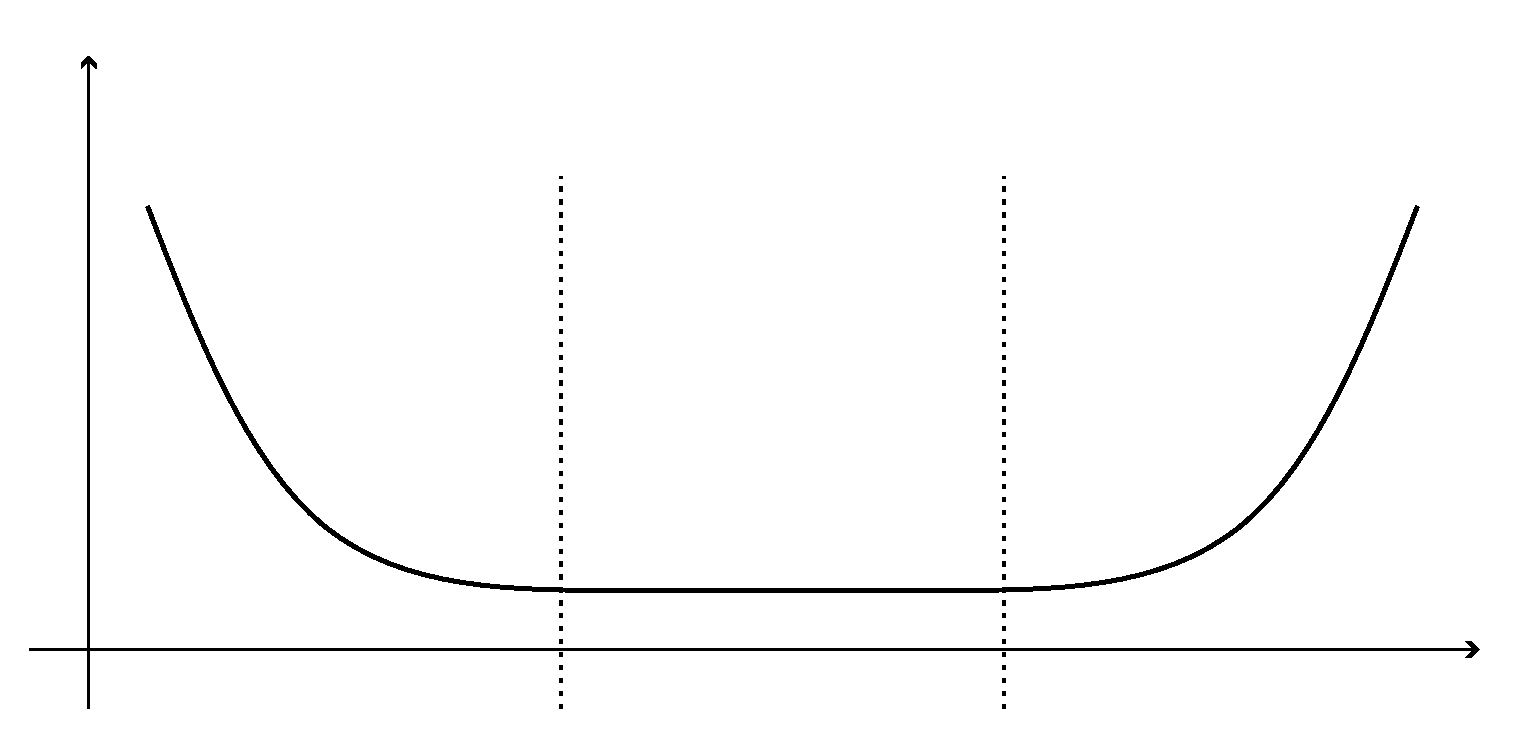
\includegraphics[width=\linewidth]{ch3_theorie_framework/abbildungen/bathtub.pdf}};
        % Koordinatensystem für die Grafik
        \begin{scope}[x={(image.south east)},y={(image.north west)}]
            % Textpositionen anpassen:
            \node at (0.25,0.92) {\large\parbox{6cm}{Ausfallwahrscheinlichkeit}};
            \node at (0.88,0.05) {\large\centering Betriebsdauer};
            \node at (0.25,0.6) {\large\parbox{4cm}{\centering I\\Frühausfälle}};
            \node at (0.51,0.6) {\large\parbox{6cm}{\centering II\\normale Lebensdauer}};
            \node at (0.77,0.6) {\large\parbox{4cm}{\centering III\\Alterserscheinungen}};
        \end{scope}
    \end{tikzpicture}
    \caption{Badewannenkurve zur Visualisierung der Ausfallverteilung}
~\label{fig:bathtub}
\end{figure}

\subsection{Predictive Maintenance}
Nach Mobley~\Cite[S.~4]{Mobley2002} wird Predictive Maintenance als eine zustandsbasierte Wartungsstrategie definiert, die den
tatsächlichen Betriebszustand von Anlagen und Systemen überwacht, um Wartungsaktivitäten bedarfsgerecht zu planen.
Eine passende Analogie findet sich in der Medizin: Wenn der menschliche Körper Anzeichen einer bevorstehenden Krankheit zeigt, können
diese Symptome vom Arzt genutzt werden, um eine Diagnose zu stellen. Dementsprechend werden dann Maßnahmen ergeriffen, zum Beispiel
wird eine Behandlung eingeleitet oder Medikamente verordnet. Diese Zustandsüberwachung erlaubt es, dass Wartungsarbeiten zu einem
Zeitpunkt stattfinden können, der für alle Beteiligten passend ist und minimale Einschnitte in Produktions- oder Prozesslaufzeiten
bedeutet~\cite[S.~3]{Scheffer2004}.

Anhand von \hyperref[fig:pdm_workflow]{Abb.~\Ref*{fig:pdm_workflow}} ist zu erkennen, welche vereinfachten Schritte zur erfolgreichen
Implementierung eines Predictive Maintenance Systems erforderlich sind. Essentiell ist an erster Stelle eine adäquate Infrastruktur, die
sämtliche Zustandsparameter erfasst und gleichzeitig in der Lage ist, die erfassten Daten auch bereitzustellen. Es müssen im nächsten
Schritt Daten gesammelt werden, damit die im normalen Betriebszustand gültigen Schwellwerte ermittelt und festgelegt werden können.
Anhand dieser wird dann im laufenden, mittlerweile aufgenommenen Betrieb festgestellt, ob Abweichungen von den Parametern im Normalbetrieb
vorliegen. Demnach werden notwendige Wartungsarbeiten geplant und vorbereitet, wonach der Betrieb wieder ordnungsgemäß aufgenommen werden
kann.

\begin{figure}[H]
    \centering
    \begin{tikzpicture}
        \node[anchor=south west,inner sep=0] (image) at (0,0) {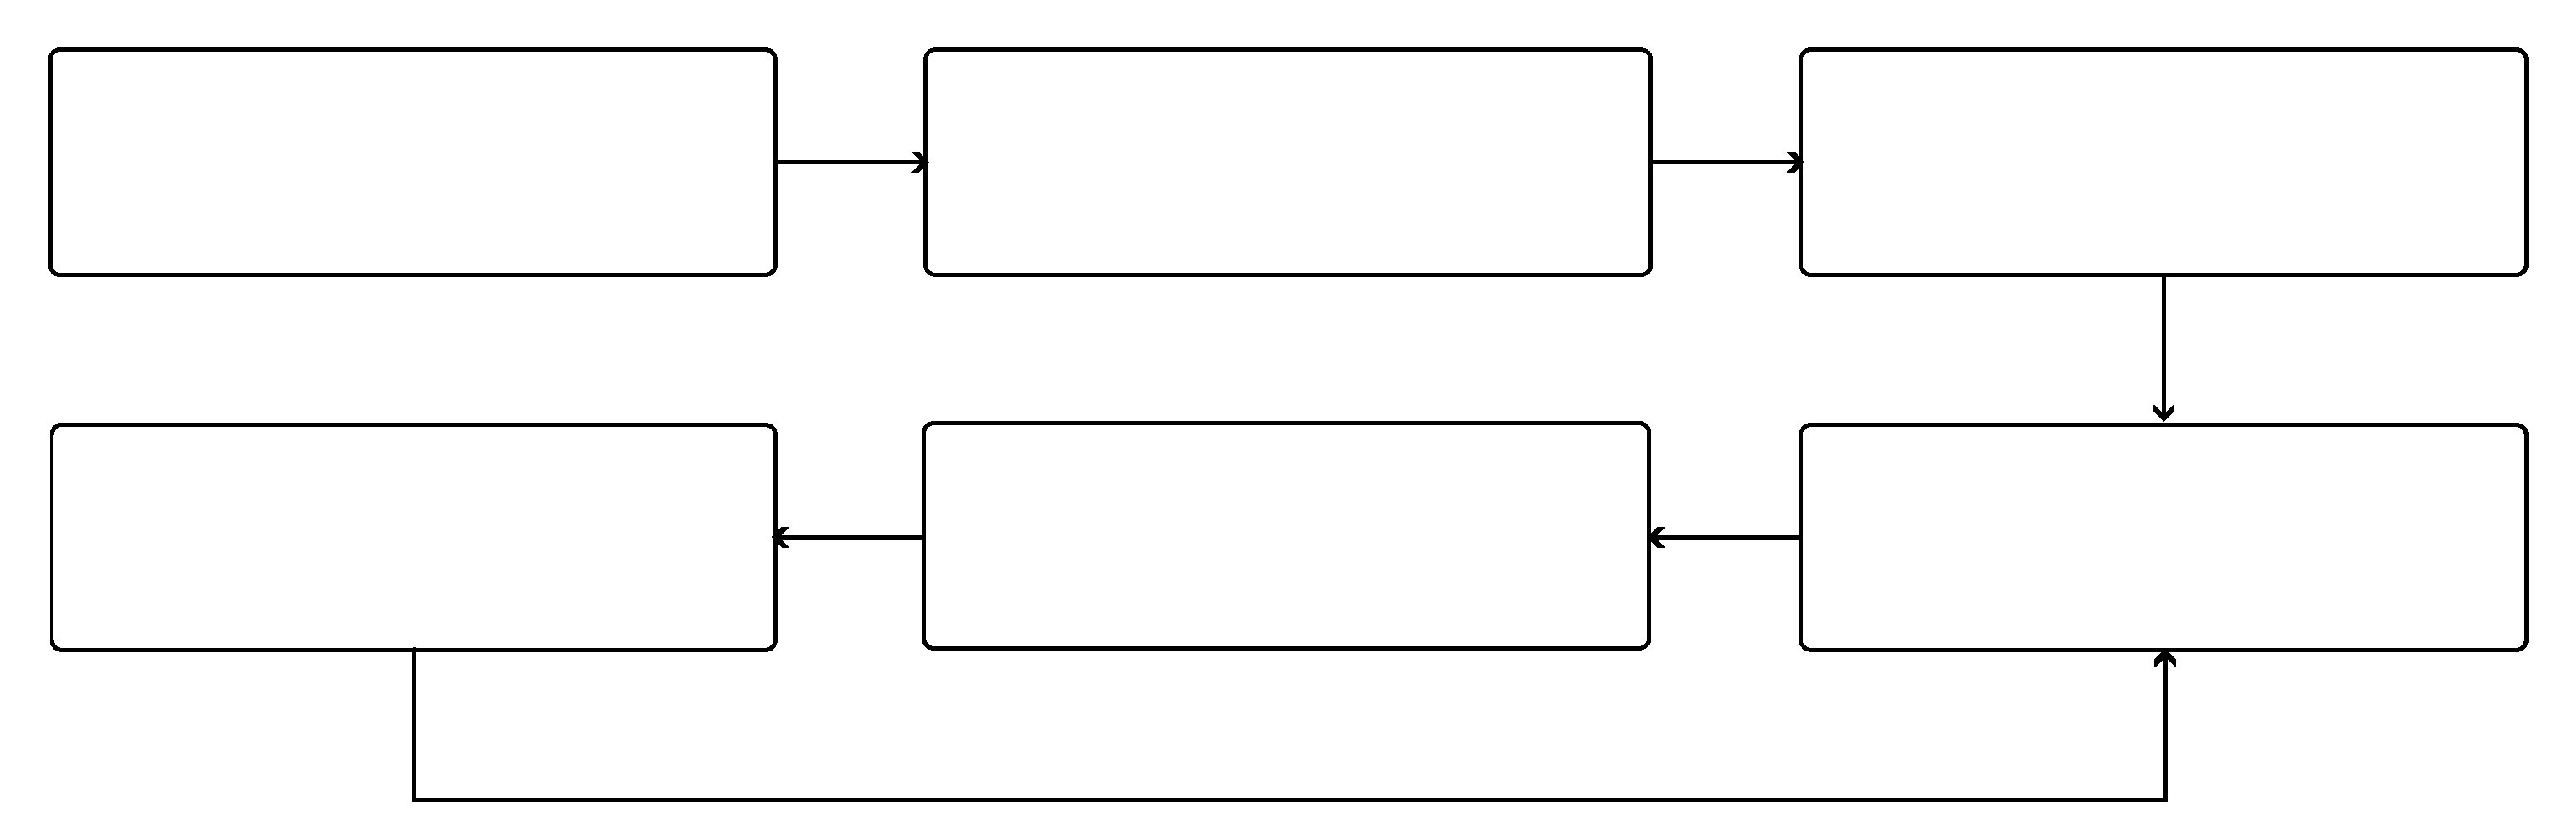
\includegraphics[width=\linewidth]{ch3_theorie_framework/abbildungen/pdm_workflow.pdf}};
        % Koordinatensystem für die Grafik
        \begin{scope}[x={(image.south east)},y={(image.north west)}]
            % Textpositionen anpassen:
            \node at (0.16,0.815) {\large\parbox{6cm}{\centering Zustandsüberwachung\\einrichten}};
            \node at (0.5,0.815) {\large\parbox{6cm}{\centering Daten aggregieren}};
            \node at (0.84,0.815) {\large\parbox{6cm}{\centering Schwellwerte festlegen \&\\Parameter setzen}};
            \node at (0.84,0.35) {\large\parbox{6cm}{\centering normale\\Betriebsaufnahme}};
            \node at (0.5,0.35) {\large\parbox{6cm}{\centering Anomalien im\\Betrieb feststellen}};
            \node at (0.16,0.35) {\large\parbox{6cm}{\centering Wartungsarbeiten\\durchführen}};
        \end{scope}
    \end{tikzpicture}
    \caption{Workflow eines Predictive Maintenance Systems}
~\label{fig:pdm_workflow}
\end{figure}

Es stellt sich die Frage, welcher Anwendungsfall hauptsächlich interessant ist. In~\hyperref[ch:zielsetzung]{Kap.~\Ref*{ch:zielsetzung}}
wird bereits erläutert, in welchem Umfang eine Diagnose bzw.~Prognose gestellt werden soll. Vorrangig ist die Detektion von anomalem
Verhalten im laufenden Betrieb wie z.~B.~auftretende Alterserscheinungen oder Komponentenausfälle. Anhand dieser Anomalien soll durch
zusätzlichen menschlichen Input entschieden werden, ob und wann ein Wartungseinsatz notwendig ist.

Predictive Maintenance ist keineswegs eine neue Erscheinung. Der Ansatz und erste Methoden zur Umsetzung bestehen bereits seit den 70er
und 80er Jahren~\cite{Sandtorv1973, Renwick1985} mit Techniken wie beispielsweise der Vibrationsanalyse zur Zustandsbestimmung. Dabei
entwickelte sich der Fokus von Predictive Maintenance von lediglich der anfänglichen Überwachung durch die immer größer werdenden
Datenmengen hin zur ganzheitlichen Zustandsüberwachung. Durch technologische und industrielle Fortschritte wie Industrie 4.0 und dem
Internet of Things wurde die Umsetzung und Implementierung von Predictive Maintenance immer einfacher und kostengünstiger. Auf diese sog.
\textit{Enabling Technologies} wird in~\hyperref[sec:technologische_grundlagen]{Abs.~\Ref*{sec:technologische_grundlagen}} genauer
eingegangen.

Insgesamt zeigt sich das Konzept der Predictive Maintenance als natürliche Weiterentwicklung der traditionellen Wartungsansätze aufgrund
der einhergehenden technologischen Fortschritte. Während diese Arbeit lediglich Teilschritte zur Entwicklung eines Predictive Maintenance
Systems beitragen will, soll anhand der Erkenntnisse und Ergebnisse die Einführung und Nutzung eines solchen Systems die offensichtliche
Konsequenz sein.

\section{Framework}\label{sec:framework}
Die Notwendigkeit und Bedeutung eines Predictive Maintenance Systems wurde nun in~\hyperref[ch:pdm_theorie]{Kap.~\Ref*{ch:pdm_theorie}}
beleuchtet, sowie der Fokus der Arbeit. Daher steht die Entwicklung eines funktionierenden Sytsems zur Anomaliedetektion an erster Stelle.
In Anlehnung an Krupitzer et al.~\cite{Krupitzer2020} werden für die Entwicklung einer Predictive Maintenance Lösung im Kontext des SSPX1
Mautüberwachungssystems einige Rahmenbedingungen skizziert. Diese lassen sich gem.
\hyperref[fig:pdm_framework]{Abb.~\Ref*{fig:pdm_framework}} kategorisieren und werden in diesem Kapitel näher beschrieben und offengelegt.
Die Zielsetzung wurde bereits in~\hyperref[ch:zielsetzung]{Kap.~\Ref*{ch:zielsetzung}} erläutert und wird daher in diesem Kapitel nicht
noch einmal besprochen.

\begin{figure}[H]
    \centering
    \begin{tikzpicture}
        \node[anchor=south west,inner sep=0] (image) at (0,0) {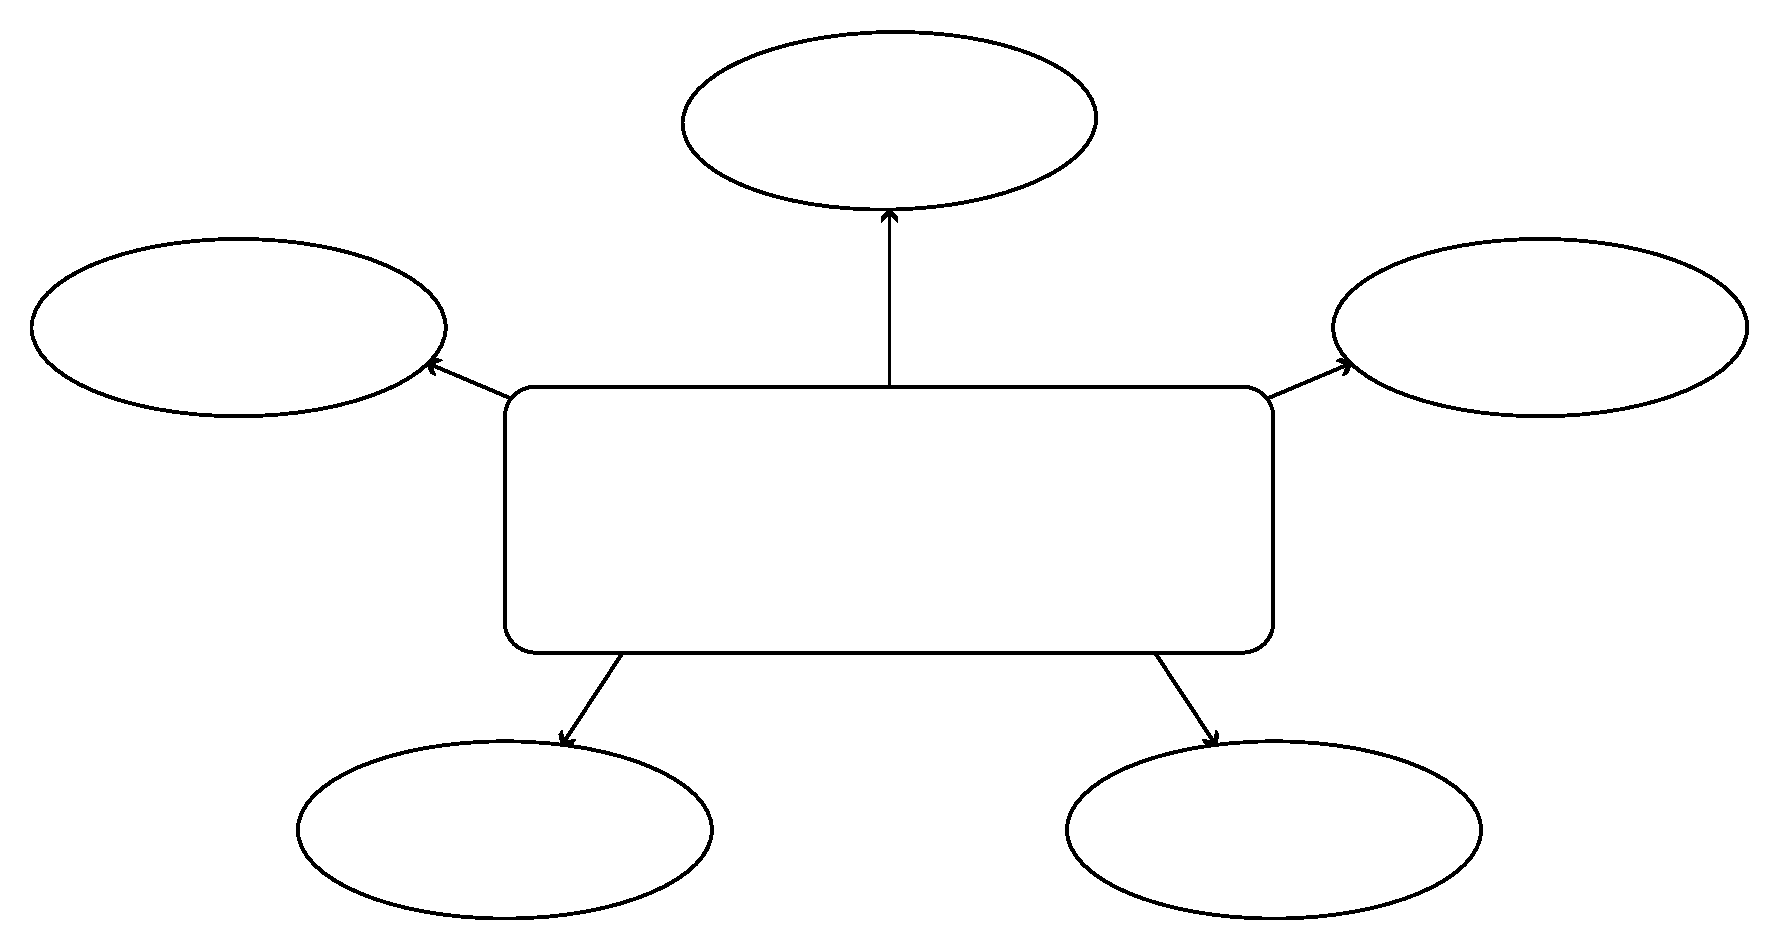
\includegraphics[width=\linewidth]{ch3_theorie_framework/abbildungen/framework.pdf}};
        % Koordinatensystem für die Grafik
        \begin{scope}[x={(image.south east)},y={(image.north west)}]
            % Textpositionen anpassen:
            \node at (0.5,0.45) {\LARGE\parbox{8cm}{\centering\textbf{Framework\\Anomaliedetektion}}};
            \node at (0.13,0.65) {\large Evaluation};
            \node at (0.87,0.65) {\large \parbox{3cm}{\centering\hyperref[sec:technologische_grundlagen]{Technologische\\Grundlagen}}};
            \node at (0.5,0.87) {\large\hyperref[ch:zielsetzung]{Zielsetzung}};
            \node at (0.28,0.13) {\large \parbox{3cm}{\centering\hyperref[sec:datenverarbeitung]{Daten-\\verarbeitung}}};
            \node at (0.72,0.13) {\large \parbox{3cm}{\centering\hyperref[sec:zustandsueberwachung]{Zustands-\\überwachung}}};
        \end{scope}
    \end{tikzpicture}
    \caption{Framework der Entwicklung eines Systems zur Anomaliedetektion}
~\label{fig:pdm_framework}
\end{figure}

\subsection{Technologische Grundlagen}\label{sec:technologische_grundlagen}
Die technologischen Grundlagen dieser Arbeit stützen sich auf die in der SSPX1 verbauten Sensoren, die präzise Systemdaten erfassen
und kontinuierlich überwachen. Zu den erfassten Parametern gehören unter anderem die Temperatur und Auslastung von GPU und CPU,
die Auslastung des Arbeitsspeichers sowie die Strom- und Leistungsaufnahme des Blitzmoduls.

Ein zentraler Baustein ist die Nutzung moderner IoT-Technologien in Kombination mit dem industriellen Kommunikationsstandard OPC UA.\
Dieser Standard basiert auf Ethernet TCP/IP und ermöglicht einen effizienten und sicheren Zugriff auf die Sensordaten der SSPX1 und
deren Übertragung an eine Anwenderschnittstelle nach dem Client-Server-Prinzip~\cite[S.~470]{Babel2024}.

Da die Sensoren teilweise von unterschiedlichen Herstellern stammen und Messdaten in verschiedenen Formaten bereitstellen, sorgt OPC
UA für eine einheitliche und standardisierte Kommunikation. Die Daten werden dabei im kompakten \textit{OPC UA Binary}-Format~\cite{iec62541}
erfasst, wodurch eine performante und ressourcenschonende Datenübertragung ermöglicht wird. Anschließend werden die Daten an den OPC
UA-Server übermittelt und in der zugrundeliegenden SQL-Datenbank gespeichert. 

Durch diese Architektur wird eine herstellerübergreifende Interoperabilität gewährleistet, weshalb OPC UA besonders für den betrachteten
Anwendungsfall geeignet ist. Die hohe Skalierbarkeit und Erweiterbarkeit des Standards ermöglicht zudem die einfache Integration
weiterer Sensoren und Systeme, wodurch zukünftige Erweiterungen ohne grundlegende Anpassungen der bestehenden Infrastruktur möglich
sind. Diese sog.~\textit{Cyber Physical Systems} ermöglichen also die Verbindung von mechanischen Komponenten über Netzwerke und sind
essentiell für die Architektur dieser Arbeit.

Ein weiterer Vorteil der Nutzung von OPC UA liegt in der serviceorientierten Architektur, die eine flexible Kommunikation
zwischen Client und Server ermöglicht. Der Client fungiert hierbei als Kommunikationsbrücke, die Anfragen und Antworten zwischen
der Anwenderschnittstelle und dem Server verwaltet. Die OPC UA-Kommunikations-Stacks unterstützen dabei die Datenverarbeitung und
gewährleisten eine robuste Übertragung, indem sie eng mit dem Speicher- und Dateisystem des Servers zusammenarbeiten. Zu den
wesentlichen Ereignissen der Client-Server-Kommunikation gehören~\cite{Babel2024,iec62541,Mao2024}:
\begin{itemize}
    \item \textbf{Message Requests:} Anfragen des Clients zur Datenabfrage oder -übertragung
    \item \textbf{Message Responses:} Antworten des Servers auf die Anfragen des Clients
    \item \textbf{Order Requests:} Aufrufe zur Ausführung bestimmter Serveraktionen
    \item \textbf{Notifications:} Benachrichtigungen über Änderungen oder Ereignisse im System
\end{itemize}

Darüber hinaus kann der OPC UA-Server als Bindeglied zwischen mehreren physischen Geräten oder auch als Cloud-Service fungieren,
was die Skalierbarkeit weiter erhöht und die Nutzung in verteilten Systemen erlaubt. Im Rahmen dieser Arbeit wird auf diese Funktionalität
jedoch verzichtet, da jedes SSPX1 Gerät einen eigenen Server betreibt, der sämtliche aufgenommenen Messdaten bereitstellt.

\subsection{Zustandsüberwachung}\label{sec:zustandsueberwachung}
Ein wesentlicher Grund für ineffiziente Wartungsmaßnahmen liegt im unzureichenden Zugang zu Daten, die frühe Hinweise auf
potenzielle Schäden oder Ausfälle liefern könnten~\cite[S.~2]{Mobley2002}. Predictive Maintenance basiert auf der Voraussetzung, dass
Daten über den Zustand des betreffenden Systems oder der betreffenden Komponente zuverlässig verfügbar sind. Die Bereitstellung der
Daten erfolgt wie oben beschrieben mithilfe von OPC UA und die Zustandsüberwachung sensorbasiert.

Zu Beginn der Arbeit und in der Entwicklungsphase wird die Zustandsüberwachung einen inspektionsbasierten Ansatz verfolgen. Das
bedeutet, dass nach willkürlichen oder festelegten Intervallen immer auf die vom OPC UA Server zur Verfügung gestellten Daten
zugegriffen wird und diese Datensätze dann analysiert und weiterverarbeitet werden. Die Wahl dieser Methode basiert auf der
geringeren Komplexität der Implementierung in frühen Entwicklungsphasen und hat zur Folge, dass ein konsistenter Datensatz einen
besseren Vergleich und Feinabstimmung von Parametern der Analysetools ermöglicht.

Online Predictive Maintenance erweitert diesen Ansatz, indem sie eine Überwachung des Systemzustands in Echtzeit im laufenden Betrieb
ermöglicht. Dabei werden Daten oder andere relevante Parameter in regelmäßigen Abständen automatisch erfasst. Nicht alle erfassten
Daten werden analysiert; vielmehr wird gezielt ausgewählt, welche Informationen für die Analyse und die Ableitung von Wartungsmaßnahmen
notwendig sind~\cite{Lindstroem2017}. 
% hier könnte man zu einem späteren zeitpunkt schreiben, wie genau die zustandsüberwachung durchgeführt wurde

Die aufgenommenen Messdaten zur Zustandsüberwachung liegen als multivariate Zeitserie vor. Das bedeutet, dass alle aufgenommenen Messwerte
mit einem Zeitstempel versehen sind. Dabei besteht die Möglichkeit, die Intervalle für die Messdatenaufnahme unterschiedlich einzustellen.
Ein Temperaturwert unterliegt langsameren Schwankungen und kann daher in größeren Intervallen aufgenommen werden, als beispielsweise die
Strom- oder Leistungsaufnahme des Blitzmoduls, wo auch kurzzeitige Spitzen und Ausreißer zuverlässig erkannt werden müssen.
% Für den Moment sind jedoch alle Messintervalle gleich. auch hier: später ggf. überarbeiten

\subsection{Datenverarbeitung}\label{sec:datenverarbeitung}
Durch die kontinuierliche Aggregation von Messdaten der SSPX1 entstehen sehr große, hochdimensionale Datensätze. Jeder Datenpunkt in
der Zeitserie $S$ ist mehrdimensional. Eine Zeitserie ist eine Menge der Mächtigkeit $n$. Alle $n$ Elemente sind reellwertige
$d$~-~dimensionale Datenpunkte $S_i\,\in\,\mathbb{R}^{d}$~\cite{Schmidl2022}. Ebenfalls lässt sich eine Zeitserie $S$ der Länge $n$ und
Dimensionalität $d$ als Matrix wie in \hyperref[eq:timeseries_matrix_sum]{Gl. \Ref*{eq:timeseries_matrix_sum}a} definieren. $x_{i}^{j}$ ist
der $i$-te Skalar der $j$-ten Dimension einer Serie $S$. Für die Dimension $j={0,\dots,d}$ der Zeitserie $S$ entspricht jede Dimension
einem Messwert im Datensatz. Da es sich um eine Zeitserie handelt, entsprechen die Indizes $i={0, \dots, n}$ den Zeitstempeln der
aufgenommenen Messwerte~\cite{Wenig2024}. Desweiteren wird eine \textit{univariate} Zeitserie als eine eindimensionale Menge definiert,
während eine \textit{multivariate} Zeitserie mehrdimensionale Werte beinhaltet. Im Kontext der Arbeit sind vorrangig multivariate
Zeitserien relevant.

\begin{equation}
    S=\{\,S_1,\,S_2,\,\dots\,,\,S_n\,\}\label{eq:timeseries_set}
\end{equation}

\begin{equation}
    \setcounter{equation}{1}
        \begin{subequations}
        \setlength{\arraycolsep}{1em}
        \renewcommand{\arraystretch}{1.5}
        \begin{aligned}
            S &=
            \begin{bmatrix} 
                x_{0}^{0} & \cdots & x_{0}^{d} \\
                \vdots & \ddots & \vdots \\
                x_{n}^{0} & \cdots & x_{n}^{d} 
            \end{bmatrix} 
            && \text{(a)} \\[1.5em]
            S &= \sum_{i=0}^{n}\,\sum_{j=0}^{d}\,x_{i}^{j} \cdot E_{ij}
            && \text{(b)}\\[1.5em]
            E_{32} &=
            \begin{bmatrix}
                0 & 0 & 0 & 0 \\
                0 & 0 & 0 & 0 \\
                0 & 1 & 0 & 0 \\
                0 & 0 & 0 & 0 \\
            \end{bmatrix}
            && \text{(c)} \\[1.5em]
        \end{aligned}
    \end{subequations}
\label{eq:timeseries_matrix_sum}
\end{equation}

Alternativ kann die Zeitserie $S$ gem.~\hyperref[eq:timeseries_matrix_sum]{Gl. \Ref*{eq:timeseries_matrix_sum}b} auch als Linearkombination
von Standardmatrizen geschrieben werden~\cite[S.~8]{Voigt2012}. Die elementweise Darstellung beschreibt die Matrix $S$ als Summe von
gewichteten Standardmatrizen $E_{ij}$, wobei jede Standardmatrix $E_{ij}$ genau an der Position $(i,j)$ den Wert 1 hat und sonst 0 ist.
\hyperref[eq:timeseries_matrix_sum]{Gl.~\Ref*{eq:timeseries_matrix_sum}c} verdeutlicht dies beispielhaft an der 4$\times$4 Einheitsmatrix
$E_{32}$.

\begin{figure}[t!]
    \centering
    \begin{tikzpicture}
        \node[anchor=south west,inner sep=0] (image) at (0,0) {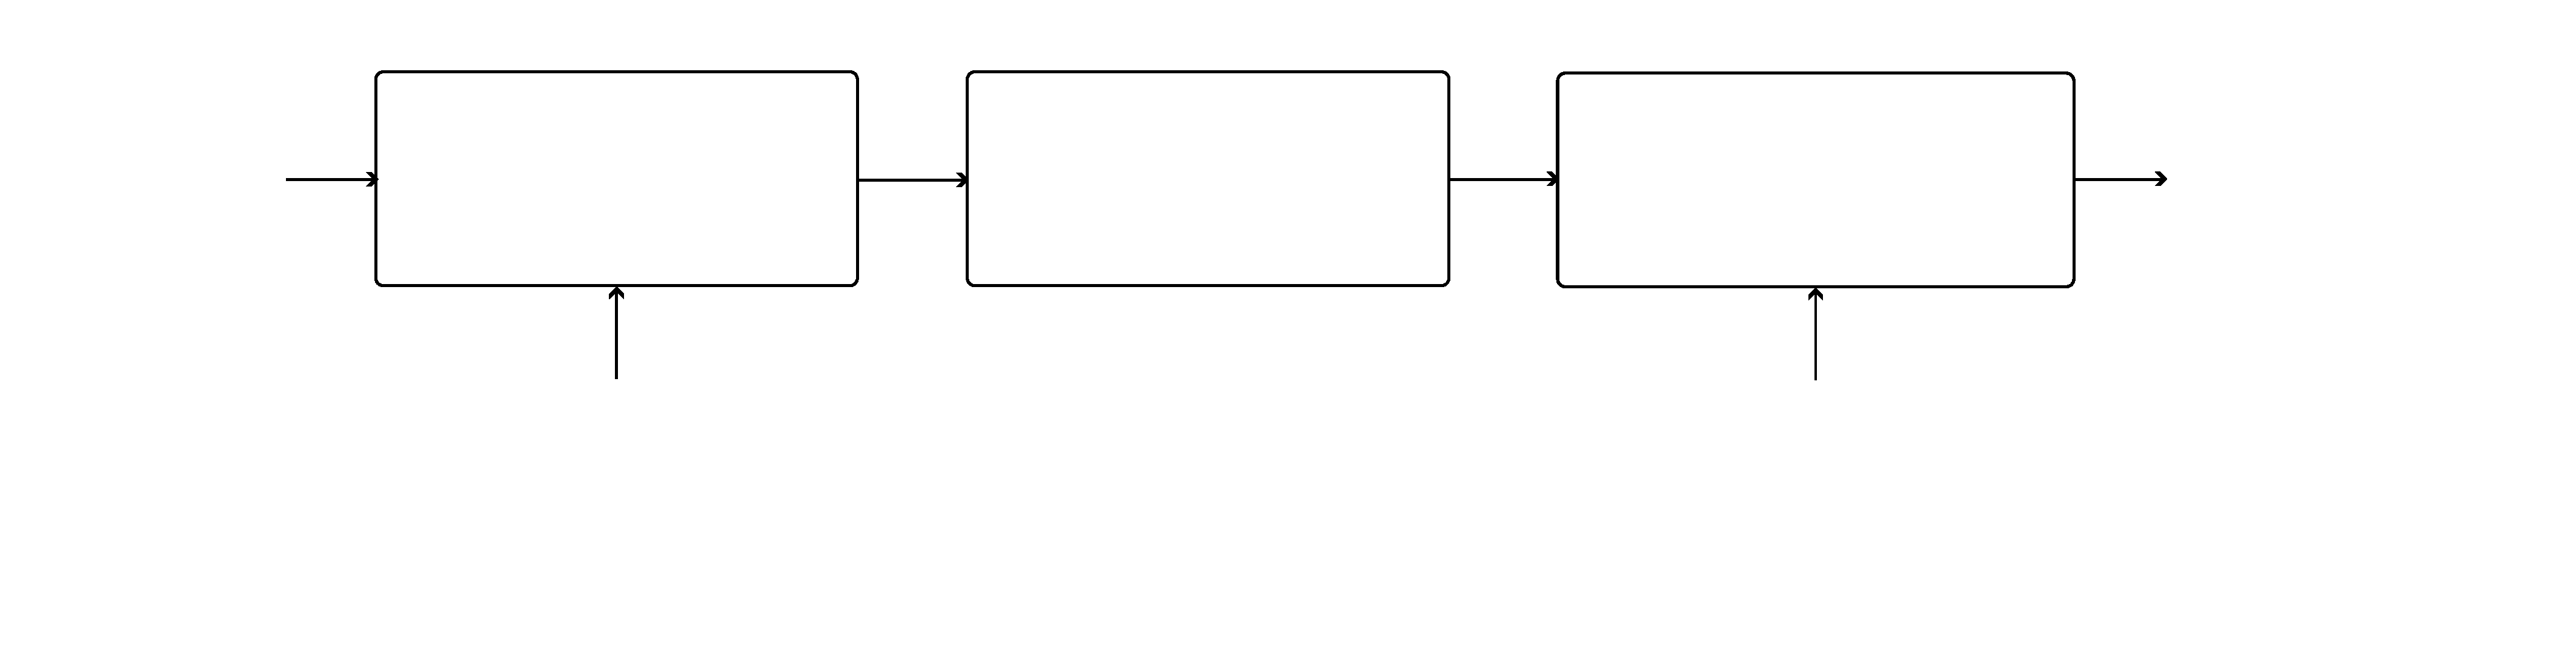
\includegraphics[width=1\linewidth]{ch3_theorie_framework/abbildungen/data_mining.pdf}};
        % Koordinatensystem für die Grafik
        \begin{scope}[x={(image.south east)},y={(image.north west)}]
            % Textpositionen anpassen:
            \node at (0.059,0.725) {\large\centering Rohdaten};
            \node at (0.2365,0.725) {\large \parbox{6cm}{\centering Vorverarbeitung\\der Daten}};
            \node at (0.47,0.725) {\large Data Mining};
            \node at (0.705,0.725) {\large \parbox{6cm}{\centering Nachverarbeitung\\der Daten}};
            \node at (0.904,0.725) {\large \parbox{3cm}{\centering Information}};
            \node at (0.2365,0.2) {\large \parbox{6cm}{\centering Dimensionalität reduzieren\\Normierung\\Subsets bilden}};
            \node at (0.705,0.2) {\large \parbox{6cm}{\centering Visualisierung\\Anomaliedetektion\\Anomalien bewerten}};
        \end{scope}
    \end{tikzpicture}
    \caption{\centering Typischer Data Mining Workflow vom Eingang der Quelldaten bis zum Informationsgewinn}
~\label{fig:data_mining}
\end{figure}

\textit{Data Mining} spielt in dem Zusammenhang eine große Rolle. Unter Data Mining versteht man das Finden relevanter Informationen,
Muster oder Trends in großen Datensätzen. Mithilfe verschiedener Data Mining Techniken können so Voraussagen über künftige Ereignisse oder
Beobachtungen getroffen werden. Der Prozess des Data Minings lässt sich anhand von~\hyperref[fig:data_mining]{Abb.~\Ref*{fig:data_mining}}
visualisieren. Dabei gehen zunächst Rohdaten aus den zahlreichen Sensoren hervor und liegen bedingt durch das SQL-Format in einer
relationalen Datenbank vor. Der nächste Schritt der Vorverarbeitung erfolgt dann, damit die Daten in einem handlichen und analysierbaren
Format vorliegen. Daher werden diese sowohl in ihrer Dimensionalität reduziert als auch normiert. Gegebenenfalls werden auch
kontextbezogene Subsets gebildet, z.~B.~für Tageszeiten oder sonstige Bedingungen~\Cite[Kap.~1]{Tan2014}.

Zur Datenverarbeitung gehören auch spezifische Herausforderungen, die die Entwicklung neuer Data Mining Techniken vorangetrieben haben.
Dazu gehört unter Anderem die Skalierbarkeit eines Algorithmus, um zu gewährleisten, dass auch sehr große und immer größer werdende
Datensätze mit der gleichen Präzision und Qualität verarbeitet werden. Desweiteren zählen auch die Hochdimensionalität und Heterogenität
der vorliegenden Datensätze zu großen Herausforderung bei der Findung geeigneter Algorithmen. Für hochdimensionale Daten muss im Voraus
im Rahmen der Vorverarbeitung eine Reduzierung der Dimensionalität stattfinden, d.h.~irrelevante oder redundante Datenpunkte werden
entfernt oder mit ähnlichen Datenpunkten zusammengefasst. Auch statistische Abhängigkeiten und Unabhängigkeiten sowie Korrelationen
werden in diesem Schritt mit berücksichtigt. Die Heterogenität eines Datensatzes zeigt sich beispielsweise durch das Auftreten von
Datenpunkten mit unterschiedlichen physikalischen Einheiten, wie Temperaturwerte und solche zur Festplattenauslastung und
-schreibgeschwindigkeit. Bevor ein Datensatz also einem Algorithmus zur Anomaliedetektion übergeben werden kann, muss eine adäquate
Vorverarbeitung stattfinden, denn nur so können auch relevante Ergebnisse erzeugt werden.

% weitere inhalte dieses abs.: wie wird die dimensionalität zb verringert? pca oder ähnliche verfahren. abhängig von den gewählten
% algorithmen, die getestet werden sollen

\newpage
\subsection{Evaluation}
% hier soll kurz vorgestellt werden, anhand welcher kriterien und mit welchen verfahren ein algorithmus bewertet werden soll
% zb. rechendauer, anomaliequote etc.
\newpage
 % chktex-file 44
 % chktex-file 24
 % chktex-file 1
 \chapter{Anomaliedetektion}\label{ch:anomaliedetektion}
Anomaliedetektion beschreibt die Aufgabe, Trends, Muster und Punkte in einem Datensatz zu finden, die nicht dem Normalzustand
entsprechen~\cite{Chandola2009}. Anders gesagt lautet das Ziel: die Punkte finden, die sich von den anderen Punkten im Datensatz
stark unterscheiden~\cite[Kap.~10]{Tan2014}. Diese andersartigen Datenpunkte oder -sequenzen werden in der Regel als Anomalie,
Ausreißer oder Ausnahmen bezeichnet, wobei Anomalie der geläufigste Begriff ist. Anomaliedetektion findet große Verwendung in
verschiedenen Anwendungsbereichen, wie z.~B.~in der Netzwerktechnik zur Erkennung von potenziellen Angriffen durch Eindringlinge
in ein Netzwerk anhand von ungewöhnlichem Traffic~\Cite{Bernacki2015}. Auch in der Medizin können nach einem Elektrokardiogramm
(\textit{EKG}) durch Anomaliedetektion Herzrhythmusstörungen erkannt werden~\cite{Chuah2007}, genau wie eine Bank ein Interesse
an Anomalien im Kreditkartenverhalten ihrer Kunden hat, um Betrugsfälle zu erkennen~\cite{Jiang2023, CeronmaniSharmila2019}.

Die simpelste Herangehensweise zur Erkennung von Anomalien ist die, dass zuerst definiert wird, welche Punkte im Datensatz normalem
Verhalten entsprechen und alle davon abweichenden Punkte als Anomalie zu kennzeichnen. Doch so einfach die Herangehensweise wirkt,
so anfällig ist sie auch für Fehler. Dabei heben sich einige Herausforderungen hervor.

Zum Einen die Frage, wo genau die Grenze zwischen normalem und anomalem Verhalten liegen soll. Eine Region zu definieren, die jeden 
möglichen normalen Punkt beinhaltet und jedmöglichen anomalen Punkt ausschließt, ist nicht trivial und oft nicht präzise durchführbar.
So ist es durchaus möglich, dass in manchen Fällen anomale Punkte als normal bezeichnet werden, und normale Punkte als anomal, je
nachdem, wo die Grenze liegt.

Es stellt sich ebenfalls die Frage, ob eine Anomalie einer binären Natur unterliegt: Entweder es handelt sich um eine Anomalie oder
einen Normalzustand. Doch die Wahrheit liegt oft in der Mitte. Weicht ein Punkt oder eine Sequenz bereits nur leicht vom Normal ab,
so kann es bereits erste Hinweise auf mögliches zukünftiges anomales Verhalten in einer Zeitserie geben, bevor sich solche Datenpunkte
als Anomalie zeigen. Deshalb ist es hilfreich, charakterisieren zu können, wie weit der Punkt oder die Sequenz
vom Normal abweicht. Diese Charakterisierung kann dabei als \textit{Anomaly Score} bezeichnet werden und beispielsweise eine Dezimalzahl
zwischen 0 und 1 sein.

Normalzustände sind in Zeitserien oft zeitvariant und daher schwer festzuhalten bei einer kontinuierlichen Datenaufzeichnung.
Zudem sind Normalzustände und Abweichungen davon in unterschiedlichen Bereichen auch unterschiedlich signifikant. Während beim
menschlichen Körper eine geringe Abweichung der Körpertemperatur bereits gravierend sein kann, ist die gleiche relative Abweichung
in einer anderen Domäne wie in einem Aktienkurs weniger drastisch und unterliegt dementsprechend auch einem Anpassungsbedarf, bevor
es an die Erkennung möglicher Anomalien geht.

Daraus lässt sich direkt zum nächsten Problem übergehen. Die Unterscheidung zwischen globalen und lokalen Anomalien~\cite{Breunig2000}.
Hier ist der Kontext wichtig: Eine Person mit einer Körpergröße von mehr als 2 $m$ ist in ihrer Nachbarschaft sicherlich eine Anomalie,
während sie in einem Basketballteam kaum herausragt~-~im wahrsten Sinne des Wortes. Diese Art der Anomalie wird auch als kontextuelle
Anomalie bezeichnet~\Cite[S.~12]{Wenig2024}.

\section{Anomaliearten}
Doch bevor eine Auswahl an geeigneten Verfahren oder Algorithmen zur Anomaliedetektion getroffen wird, muss zuerst verstanden werden,
welche verschiedenen Arten von Anomalien es gibt und wie sich diese voneinander unterscheiden.
Auch wenn Studien zeigen, dass es durchaus Algorithmen gibt, die über mehrere verschiedene Kategorien gut
abschneiden~\cite[S.~30~-~31]{Wenig2024}~\cite{Schmidl2022}, so soll zunächst für jede Kategorie mindestens ein passender Kandidat
gefunden werden. Diese werden dann in einem nächsten Schritt kreuzweise getestet, um auch solche Allrounder entdecken zu können. Dabei
ist auch immer der Kontext der Anwendung wichtig. Wie eingangs erwähnt, sind für verschiedene Tätigkeitsfelder verschiedene
Anforderungen an die Präzision oder Genauigkeit gestellt, weshalb immer die spezifischen Anforderung bedacht werden müssen, und nicht
jeder Algorithmus gleich performant ist über mehrere Datensätze hinweg.

Für die Kategorien wird sich zunächst auf wenige, für diese Arbeit relevante, beschränkt: \textbf{Punkt\-anomalien},
\textbf{Subsequenzanomalien} und \textbf{Korrelationsanomalien}, abgeleitet von Chandola et al.~\cite{Chandola2009}.

\subsection{Punktanomalien}
Ein einzelner Datenpunkt, der stark von den anderen Punkten im Datensatz abweicht, heißt Punkt\-anomalie~\cite{Chandola2009}. Genauer
gesagt, wenn ein Datenpunkt weit außerhalb der Wahrscheinlichkeitsverteilung des Datensatzes liegt, ist er anomal~\Cite[Kap.~10]{Tan2014}.
Punktanomalien können recht leicht erkannt werden, da Punktanomalien stark vom Mittelwert und vom Median des Datensatzes abweichen. Wenn
von Ausreißern gesprochen wird, sind damit typischerweise Punktanomalien gemeint.

Als Beispielszenario dient ein Smart Meter, das den stündlichen Stromverbrauch misst.
In~\hyperref[subfig:smartmeter]{Abb.~\Ref*{subfig:smartmeter}} ist der gemessene Stromverbrauch dargestellt mit einer klar
erkennbaren Punktanomalie am 01.08.~um 18 Uhr. Die Anomalie wird mit bloßem Auge deutlich und kann auch mit statistischen Größen
nachgewiesen werden, wie in~\hyperref[subfig:smartmeter_histogramm]{Abb.~\Ref*{subfig:smartmeter_histogramm}} anhand der
Häufigkeitsverteilung und dem Mittelwert sowie dem Median zu sehen ist. Das Histogramm dient als gute Approximation für die
Wahrscheinlichkeitsverteilung der Messwerte, und zeigt entsprechend die Eindeutigkeit des Ausreißers.

\begin{figure}[!t]
    \centering
    \begin{subfigure}[b]{0.49\linewidth}
        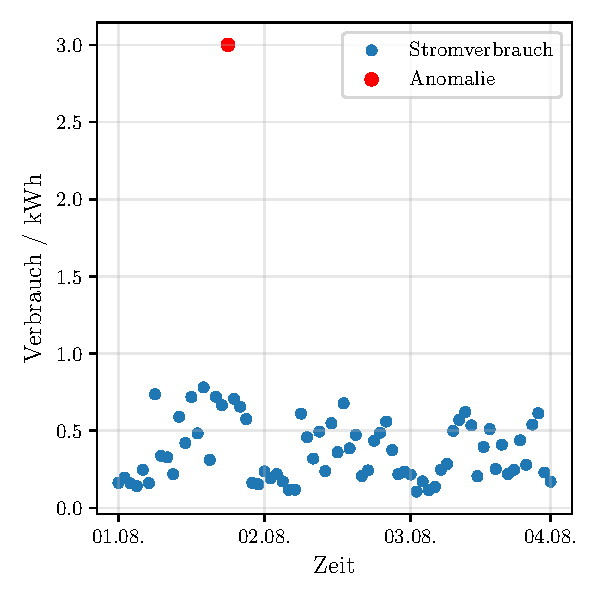
\includegraphics[width=\linewidth]{ch4_anomalien/abbildungen/punktanomalie_bsp.pdf}
        \caption{Stündliche Smart Meter Messdaten}\label{subfig:smartmeter}
    \end{subfigure}
    \begin{subfigure}[b]{0.49\linewidth}
        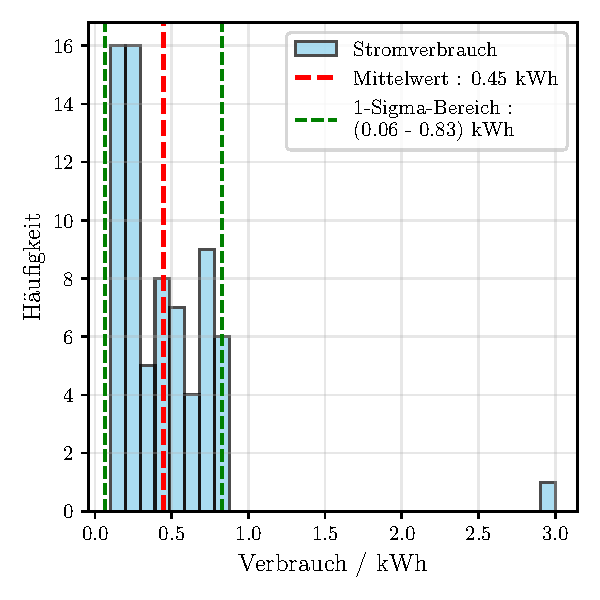
\includegraphics[width=\linewidth]{ch4_anomalien/abbildungen/punktanomalie_hist.pdf}
        \caption{\centering Histogramm des gemessenen Stromverbrauchs}\label{subfig:smartmeter_histogramm}
    \end{subfigure}
    \caption{\centering Beispielszenario einer Punktanomalie: Stromverbrauch eines Haushaltes über den Zeitraum von
    drei Tagen. Anhand des Histogramms wird die Anomalie verdeutlicht.}\label{fig:punktanomalie}
\end{figure}

Um nun eine Aussage treffen zu können, ist es wichtig den Kontext der vorliegenden Daten zu kennen. Wenn Daten für ein weitaus größeres
Zeitfenster vorliegen, z.~B.~für eine Woche oder einen Monat, könnte sich möglicherweise zeigen, dass der hohe Verbrauch öfter und
regelmäßiger vorkommt als im gezeigten Zeitraum von drei Tagen. Ob eine globale oder lediglich eine lokale Anomalie vorliegt, wird
mit einem größeren Datensatz besser erkennbar. Die Anomalie könnte beispielsweise auf das gelegentliche Betreiben einer Sauna im Haus
zurückführbar sein, dann würde es sich lediglich um eine lokale Anomalie handeln und in einem größeren Zeitraum in bestimmten Abständen
öfter vorkommen, und wäre somit keine globale Anomalie~\Cite[Kap.~10]{Tan2014}.

Punktanomalien sind im Kontext dieser Arbeit tendenziell weniger relevant, sollen aber aufgrund ihrer grundsätzlichen Bedeutung bzgl.
Anomaliedetektion als einfachste Kategorie trotzdem beleuchtet werden, um entsprechende Algorithmen, die der Erkennung solcher
Punktanomalien zuzuordnen sind, auch gegenüber anderen Anomalien zu testen.

\subsection{Subsequenzanomalien}

Eine Zeitserie wird gem.~\hyperref[eq:timeseries_set]{Gl.~\Ref*{eq:timeseries_set}} bereits als eine Menge definiert. Demnach wird eine
Subsequenz $S_{i,\,j} = \{\,S_i,\,\dots,\,S_j\,\}\,\subseteq\,S$ von der Zeitserie $S$ umfasst, mit der Länge oder Mächtigkeit
$|\,S_{i,\,j}\,|=j-i+1$ und $|\,S_{i,j}\,|\,\ge\,1$~\cite{Schmidl2022} und stellt somit einen Ausschnitt der urpsrünglichen Zeitserie
dar. Subsequenz\-anomalien sind Muster in Zeitreihen, die von anderen Mustern innerhalb der gleichen Zeitreihe
abweichen~\cite{Chandola2009}\Cite[S.~12]{Wenig2024}. Im Gegensatz zu Punktanomalien beziehen sich Subsequenz\-ano\-malien auf mehrere
konsekutive Datenpunkte, die ein ungewöhnliches Muster bilden. Eine anomale Subsequenz kann also bedeuten, dass die Datenpunkte innerhalb
der Subsequenz Werte in einem normalen, zu erwartenden Bereich annehmen, aber der zu Grunde liegende Trend ungewöhnlich
ist~\cite{Chandola2009}\cite[S.~17]{Boniol2021}. Solche ungewöhnlichen oder einzigartigen Trends und Entwicklungen können auf zukünftig
auftretende Probleme hindeuten, die sonst unentdeckt bleiben würden.

\begin{figure}[H]
    \centering
    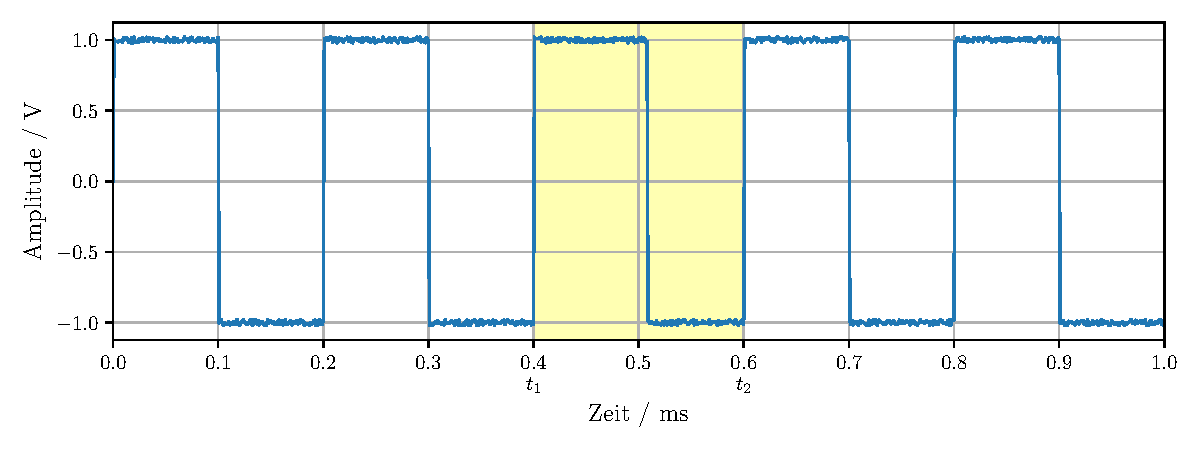
\includegraphics[width=\linewidth]{ch4_anomalien/abbildungen/subsequenz_anomalie.pdf}
    \caption{\centering Einfaches Beispiel einer Subsequenzanomalie: Rechteckspannung, die zwischen -1 und +1 V oszilliert mit einer
    Frequenz von 5 kHz. Auffällig ist die Periode zwischen $t_1=0.4\,$ms und $t_2=0.6\,$ms, bei der eine verspätete abfallende Flanke zu
    beobachten ist.}
~\label{fig:subsequenz_rect}
\end{figure}

Das Beispiel in~\hyperref[fig:subsequenz_rect]{Abb.~\Ref*{fig:subsequenz_rect}} zeigt eine sichtbare Subsequenzanomalie, die verspätete
abfallende Flanke einer gemessenen Rechteckspannung. Das Muster zwischen $t_1$ und $t_2$ ist also merklich anders verglichen zu den
restlichen 0,2 ms langen Perioden und daher eine Anomalie.

Bei der Analyse von EKG Daten spielen Subsequenzanomalien eine wichtige Rolle und können wertvolle Rückschlüsse auf die Herzgesundheit
liefern~\cite{Chuah2007}.~\hyperref[fig:ekg_herzerkrankung]{Abb.~\Ref*{fig:ekg_herzerkrankung}} zeigt EKG-Daten eines Patienten mit
monomorpher ventrikulärer Tachykardie. Diese kann zu Kammerflimmern übergehen, welches unbehandelt sogar zu einem Herzstillstand
führen kann~\cite{ekgecho}\Cite[S.~131~ff.]{Davies2015}.

\begin{figure}[h]
    \centering
    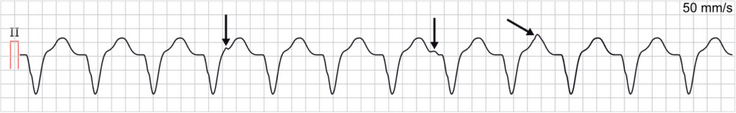
\includegraphics[width=0.85\linewidth]{ch4_anomalien/abbildungen/ventrikulaere_tachykardie.png}
    \caption{EKG Kanal mit Diagnose: Ventrikuläre Tachykardie~\cite{ekgecho}}
~\label{fig:ekg_herzerkrankung}
\end{figure}

Sichtbar sind die einzelnen Unregelmäßigkeiten im EKG Verlauf. Die Pfeile kennzeichnen die sog. P-Wellen, die Informationen darüber
liefern, dass Vorhöfe und Herzkammern nicht synchron schlagen~\cite{ekgecho}\Cite[S.~31~f.]{Davies2015}. Durch die Irregularitäten lässt
sich also erkennen, dass für den untersuchten Patienten eine Behandlung notwendig ist und betont die Wichtigkeit, diese Anomalien zu
erkennen, um wesentlich Schlimmeres zu verhindern.

Darin liegt auch eine der Herausforderungen der Subsequenzanomaliedetektion: Ab wann ist ein Trend, der so noch nicht aufgetreten ist,
Grund genug, um Maßnahmen zu ergreifen? Es bedarf also menschlicher Expertise zur Einordnung und Interpretation von Anomalien, eben wie
bei EKG Daten.

\subsection{Korrelationsanomalien}

\begin{figure}[H]
    \centering
    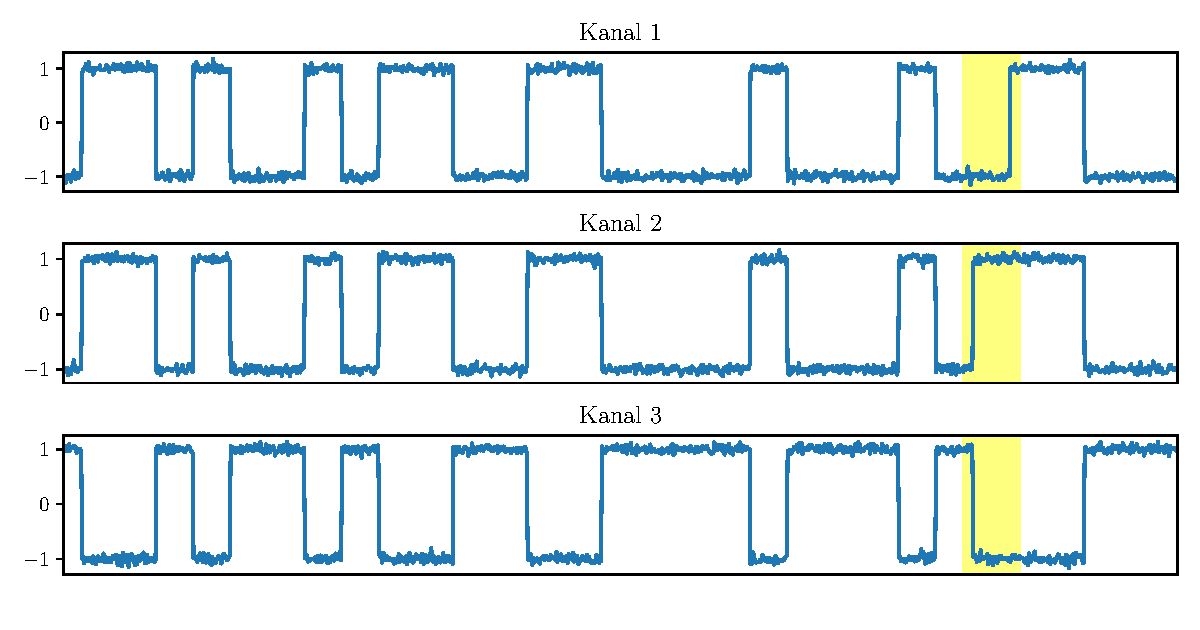
\includegraphics[width=0.95\linewidth]{ch4_anomalien/abbildungen/korrelationsanomalie.pdf}
    \caption{\centering Korrelationsanomalie zwischen Kanal 1 und den Kanälen 2 und 3 im gelb markierten Bereich. Quelle: Datensatz
        \textit{CoMuT}~\cite{NaumannCoMuT}}
~\label{fig:correlation_Anomaly}
\end{figure}

Während Punkt- und Subsequenzanomalien sowohl für univariate als auch multivariate Datensätze und Zeitserien auftreten können, sind
Korrelationsanomalien nur möglich bei zwei oder mehr Dimensionen einer Zeitreihe und betrachten die Interaktionen zwischen
verschiedenen Kanälen. Von einer Korrelationsanomalie spricht man bei Abweichungen dieser Beziehung zwischen zwei oder mehreren
Kanälen~\cite[S.12-13]{Wenig2024}~\cite{Wenig2024a}.

Im vorliegenden Beispiel in~\hyperref[fig:correlation_Anomaly]{Abb.~\Ref*{fig:correlation_Anomaly}} ist ein Auszug aus dem Datensatz
\textit{CoMuT}~- \textbf{Co}rrelated \textbf{Mu}lti\-variate \textbf{T}ime Series~\cite{NaumannCoMuT} dargestellt. Die Zeitreihe besteht
aus drei Kanälen, die zu zufälligen Zeitpunkten sprungartig ihren Wert zwischen $-$1 und 1 wechseln und jeweils leicht verrauscht sind.
Kanal 1 und 2 sind stark korreliert, während Kanal 3 stark antikorreliert zu den beiden ersten Kanälen ist. Diese Korrelation wird im
markierten Bereich verletzt, da Kanal 1 zeitlich versetzt zu den anderen beiden Kanälen springt~$-$~somit liegt eine
Korrelations\-anomalie vor.

\section{Algorithmen zur Anomaliedetektion}
In der Literatur gibt es eine breite Spanne an erprobten, möglichen Algorithmen zur Detektion der gesuchten
Anomalietypen~\cite{Schmidl2022}~\cite{BlazquezGarcia2020}~\cite{Mane2022}~\cite{Wenig2024a}. Da der zeitliche Rahmen dieser Arbeit
begrenzt ist und der vorrangige Fokus die Anwendung der Anomaliedetektionsthematik ist, müssen bei der Auswahl der Algorithmen
einige Einschränkungen vorab festgelegt werden. Dazu gehört, dass ein Algorithmus bereits implementiert wurde und optimalerweise als Open
Source Python Bibliothek o.ä.~zur Verfügung steht oder die Idee durch bereits vorhandene Komponenten einfach selbst implementiert
werden kann. Desweiteren soll es sich zu Beginn um Algorithmen handeln, die ohne vorheriges Training
auskommen, also sog. Unsupervised Learning Algorithmen. Dazu eignen sich die folgenden Techniken bzw.~Algorithmen am Besten.

\subsection{Histogram-Based Outlier Score}
Der erste Algorithmus zur Detektion von Punktanomalien ist der zur Ermittlung des \textbf{Histogram-Based Outlier Score} (HBOS), der sich
sowohl für univariate als auch multivariate Zeitserien eignet. Dabei wird für jede Dimension eine Analyse der Häufigkeitsverteilung per
Histogramm durchgeführt und anhand dessen der namensgebende Outlier Score berechnet. Die Häufigkeit aller Werte innerhalb eines Bins wird als
Dichte aufsummiert, und die Dichte ergibt gem.~\hyperref[eq:hbos]{Gl.~\Ref*{eq:hbos}} invers logarithmiert den Outlier Score. So erhalten Bins
mit geringen Häufigkeiten, also die Bins mit selten auftretenden Werten~-~wahrscheinliche Anomalien~-~einen hohen Outlier Score und können
so als Anomalie detektiert werden~\cite{Goldstein2012}.

\begin{equation}
    \text{HBOS}\,(p)\, =\, \sum_{i=0} ^ {d}\, \log \left( \frac{1}{\text{hist}_i(p)} \right)
\label{eq:hbos}
\end{equation}

Die Häufigkeitsanalyse über den kompletten Datensatz bzw.~eine sehr große Datenmenge führt dazu, dass lokale Anomalien nicht erkannt werden,
da diese Werte trotzdem innerhalb der erwarteten Verteilung liegen und im globalen Kontext nicht herausstehen,
wie~\hyperref[fig:hbos_lokale_probleme]{Abb.~\Ref*{fig:hbos_lokale_probleme}} zeigt. Einfache Abhilfe liefert die
in~\hyperref[fig:hbos_lösung]{Abb.~\Ref*{fig:hbos_lösung}} dargestellte Erweiterung um ein gleitendes Fenster variabler Größe. Der HBOS wird dann innerhalb
eines jeden Fensters ermittelt, wodurch der zeitliche Kontext mit einbezogen wird und auch lokale Anomalien erkannt werden. Multivariate Systeme
können ebenfalls einfach analysiert werden, indem für jede Variable oder Dimension separate Histogramme erstellt werden.

\begin{figure}[H]
    \centering
        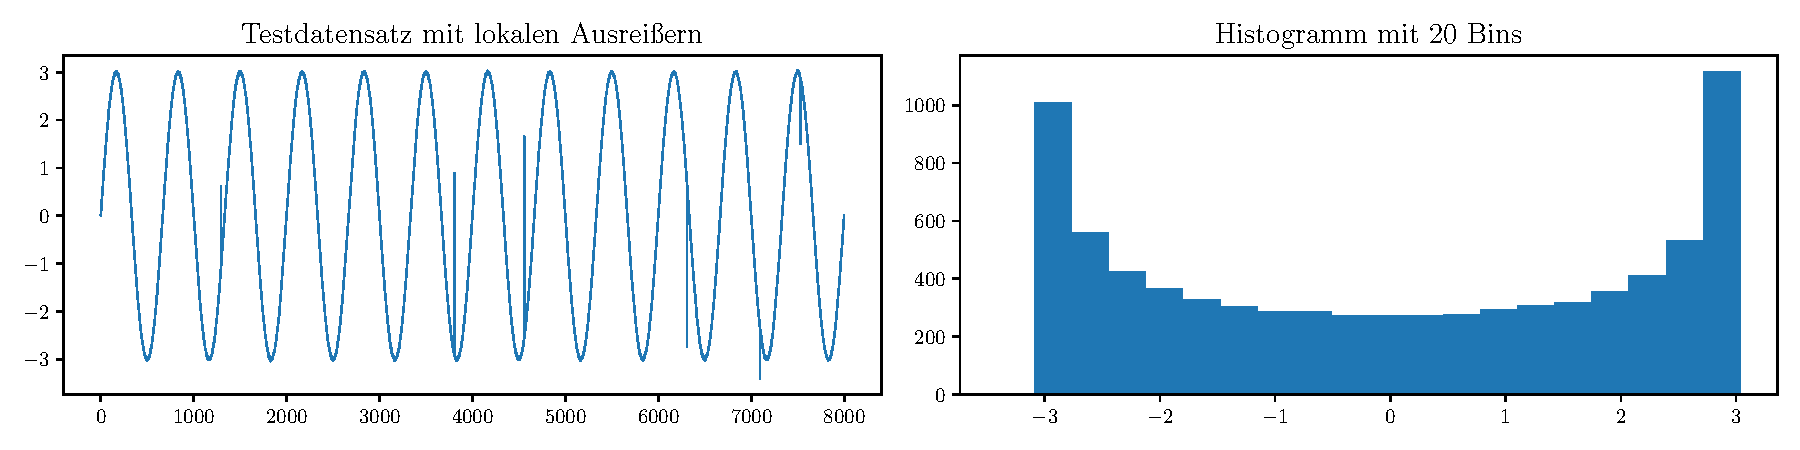
\includegraphics[width=1\linewidth]{ch4_anomalien/abbildungen/hbos_lokal_problem.pdf}    
    \caption{\centering Problematik der Detektion lokaler Punktanomalien: Da lokale Anomalien innerhalb des erwarteten Wertebereichs und damit der erwarteten
    Verteilung liegen, werde diese vom Algorithmus nicht als Ausreißer erkannt.}
~\label{fig:hbos_lokale_probleme}
\end{figure}

\begin{figure}[H]
    \centering
        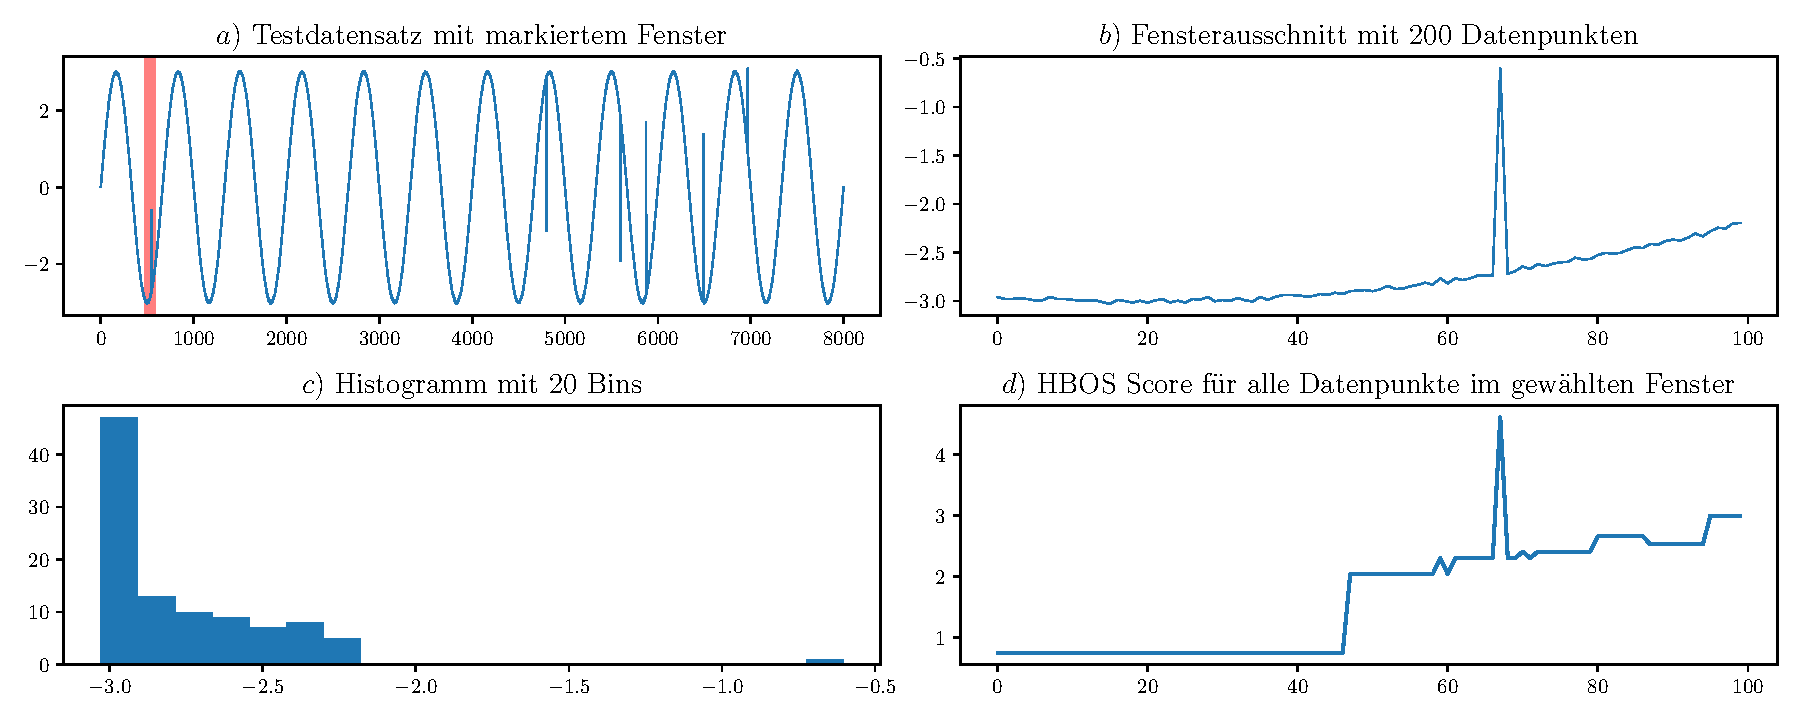
\includegraphics[width=1\linewidth]{ch4_anomalien/abbildungen/hbos_lokale_anomalien.pdf}    
    \caption{\centering Lösung der Detektionsproblematik für lokale Anomalien durch ein gleitendes Fenster. Beispielhaft dargestellt an einer Fenstergröße
    von $n=100$.}
~\label{fig:hbos_lösung}
\end{figure}

\subsection{Sliding Window Z-Score}
Durch die Berechnung eines gleitenden Mittelwerts sowie der entsprechenden gleitenden Standardabweichung kann der Z-Score eines Datenpunkts
gem.~\hyperref[eq:zscore]{Gl.~\Ref*{eq:zscore}} bestimmt werden. Der Z-Score wird in einer ähnlichen Form bereits im Jahre 1969 in \textit{Grubb's
Test} erstmals erwähnt~\cite{Grubbs1969}. Dabei bezeichnet $x_i$ den zu untersuchenden Datenpunkt, $\mu_W$ den Mittelwert und $\sigma_W$ die
Standardabweichung des Fensters~\Cite[S.~15:31]{Chandola2009}.

\begin{equation}
    Z_i\, =\, \frac{|\, x_i\,-\, \mu_W\,|}{\sigma_W}
\label{eq:zscore}
\end{equation}

Um für die Zeitserie den Zeitbezug beizubehalten, werden die statistischen Größen mit einem gleitenden Fenster berechnet, um auch lokale Ausreißer,
deren absolute Werte innerhalb der globalen Verteilung liegen, detektieren zu können. Dabei ist die Fenstergröße zunächst fest. Entsprechend des
Z-Scores deutet ein hoher Wert auf eine Anomalie hin, aufgrund der großen Abweichung zum gleitenden Mittelwert trotz Skalierung durch die
Standardabweichung. Damit ist der Z-Score eine dimensionslose Größe, die direkt als Anomaly Score interpretiert werden kann.

\subsection{GrammarViz 2.0}
Der nächste Algorithmus namens \textbf{GrammarViz} wird zur Detektion von Subsequenzanomalien eingesetzt~\cite{Senin2015}. Die Funktionsweise
basiert auf der Diskretisierung einer Zeitreihe in Symbole. Für Subsequenzen unterschiedlicher Größe wird dann versucht, diese mit
Grammatikregeln zu beschreiben. Kann sich eine Subsequenz nicht entsprechend der am häufigsten auftretenden Grammatikregeln charakterisieren
lassen, so handelt es sich wahrscheinlich um eine anomale Sequenz, beispielsweise durch ein ungewöhnliches Muster oder eine neue Trendentwicklung.

Da zum Erlernen von Grammatikregeln diskretisierte Daten benötigt werden, erfolgt die Diskretisierung in einem ersten Schritt mit dem Algorithmus SAX
(\textit{\textbf{S}ymbolic \textbf{A}ggregation Appro\textbf{X}imation}), der aus Datensätzen bzw.~-sequenzen äquivalente Symbole erzeugt~\cite{Patel}.
Aufgrund der Natur von Subsequenzanomalien wird SAX per gleitendem Fenster angewandt. Innerhalb jedes Fensters wird die Subsequenz Z-normalisiert (vgl.
Z-Scoring in~\hyperref[eq:zscore]{Gl.~\Ref*{eq:zscore}}) und anschließend in $w$ gleichwahrscheinliche Segmente diskretisiert, mit $w$ als Anzahl an
Symbolen. Durch die Z-Normalisierung folgt die Sequenz einer Gauß-Verteilung und wird
entspr.~\hyperref[tab:normalverteilung_segmente]{Tab.~\Ref*{tab:normalverteilung_segmente}} sowie am Beispiel $w=6$
in~\hyperref[fig:normalverteilung_segmente]{Abb.~\Ref*{fig:normalverteilung_segmente}} unterteilt.

\begin{table}[H]
    \centering
    \renewcommand{\arraystretch}{1.1}
    \begin{tabular}{l|rrrrrrrr}
        \backslashbox{$\beta _i$}{$w$} & 3                 & 4                   & 5                   & 6                   & 7                   & 8                   & 9                   & 10      \\
    \hline
    $\beta _1$ & $-0,43$             & $-0,67$             & $-0,84$             & $-0,97$             & $-1,07$             & $-1,15$             & $-1,22$             & $-1,28$ \\
    $\beta _2$ & $0,43$              & 0                   & $-0,25$             & $-0,43$             & $-0,57$             & $-0,67$             & $-0,76$             & $-0,84$ \\
    $\beta _3$ & \cellcolor{blue!15} & $0,67$              & $0,25$              & 0                   & $-0,18$             & $-0,32$             & $-0,43$             & $-0,52$ \\
    $\beta _4$ & \cellcolor{blue!15} & \cellcolor{blue!15} & $0,84$              & $0,43$              & $0,18$              & 0                   & $-0,14$             & $-0,25$ \\
    $\beta _5$ & \cellcolor{blue!15} & \cellcolor{blue!15} & \cellcolor{blue!15} & $0,97$              & $0,57$              & $0,32$              & $0,14$              & 0       \\
    $\beta _6$ & \cellcolor{blue!15} & \cellcolor{blue!15} & \cellcolor{blue!15} & \cellcolor{blue!15} & $1,07$              & $0,67$              & $0,43$              & $0,25$  \\
    $\beta _7$ & \cellcolor{blue!15} & \cellcolor{blue!15} & \cellcolor{blue!15} & \cellcolor{blue!15} & \cellcolor{blue!15} & $1,15$              & $0,76$              & $0,52$  \\
    $\beta _8$ & \cellcolor{blue!15} & \cellcolor{blue!15} & \cellcolor{blue!15} & \cellcolor{blue!15} & \cellcolor{blue!15} & \cellcolor{blue!15} & $1,22$              & $0,84$  \\
    $\beta _9$ & \cellcolor{blue!15} & \cellcolor{blue!15} & \cellcolor{blue!15} & \cellcolor{blue!15} & \cellcolor{blue!15} & \cellcolor{blue!15} & \cellcolor{blue!15} & $1,28$ 
    \end{tabular}
\caption{\centering z-Werte einer Normalverteilung für Segmente mit gleichem Flächeninhalt ergo gleicher Wahrscheinlichkeit. $\beta _i$ mit
$1 \le i \le w-1$ sowie $\beta _0=-\infty$ und $\beta _w=+\infty$ entsprechen den z-Koordinaten für die jeweilige Aufteilung der z-Achse.
Quelle:~\cite{Patel}}
~\label{tab:normalverteilung_segmente}
\end{table}

\begin{figure}[t!]
    \centering
        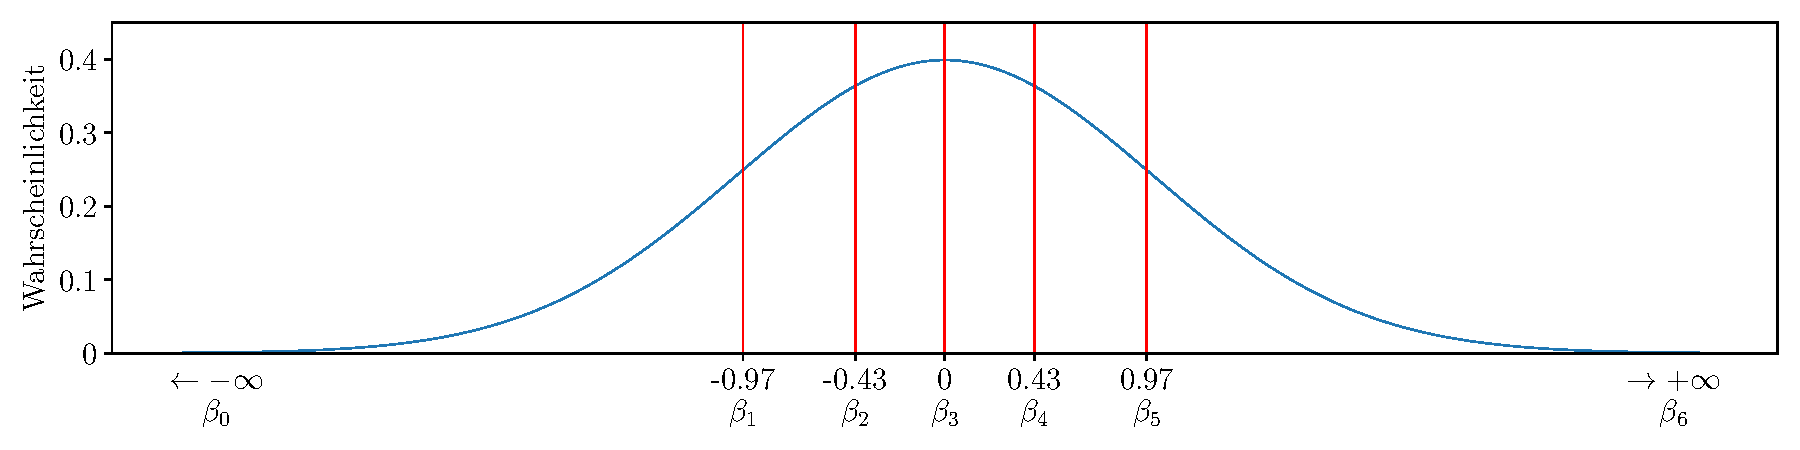
\includegraphics[width=\linewidth]{ch4_anomalien/abbildungen/normalverteilung_SAX_segmente.pdf}
    \caption{Normalverteilung mit $w=6$ gleichwahrscheinlichen Segmenten gem.~\hyperref[tab:normalverteilung_segmente]{Tab.~\Ref*{tab:normalverteilung_segmente}}}
~\label{fig:normalverteilung_segmente}
\end{figure}

Die diskretisierte Subsequenz produziert dann eine Menge an SAX Worten, die mit dem Grammatikinferenzalgorithmus Sequitur~\cite{NevillManning1997}
weiterverarbeitet werden, um rekursiv kontextfreie Grammatikregeln aufzustellen. Mithilfe einer GUI kann ein Datensatz analysiert werden und mit der
erzeugten \textbf{Rule Density Curve} sowie den einzeln aufgelisteten potenziell anomalen Sequenzen untersucht werden. Die Rule Density Curve gibt Aufschluss
darüber, wieviele Grammatikregeln pro Datenpunkt greifen. Das heißt anschaulich: je mehr Grammatikregeln, desto normaler ist ein Datenpunkt bzw.~eine
Subsequenz~\cite{senin-gv2}.

\subsection{Sliding Window Isolation Forest Density}
\label{subsec:swifd}

\begin{figure}[b!]
    \centering
    \begin{tikzpicture}
        \node[anchor=south west,inner sep=0] (image) at (0,0) {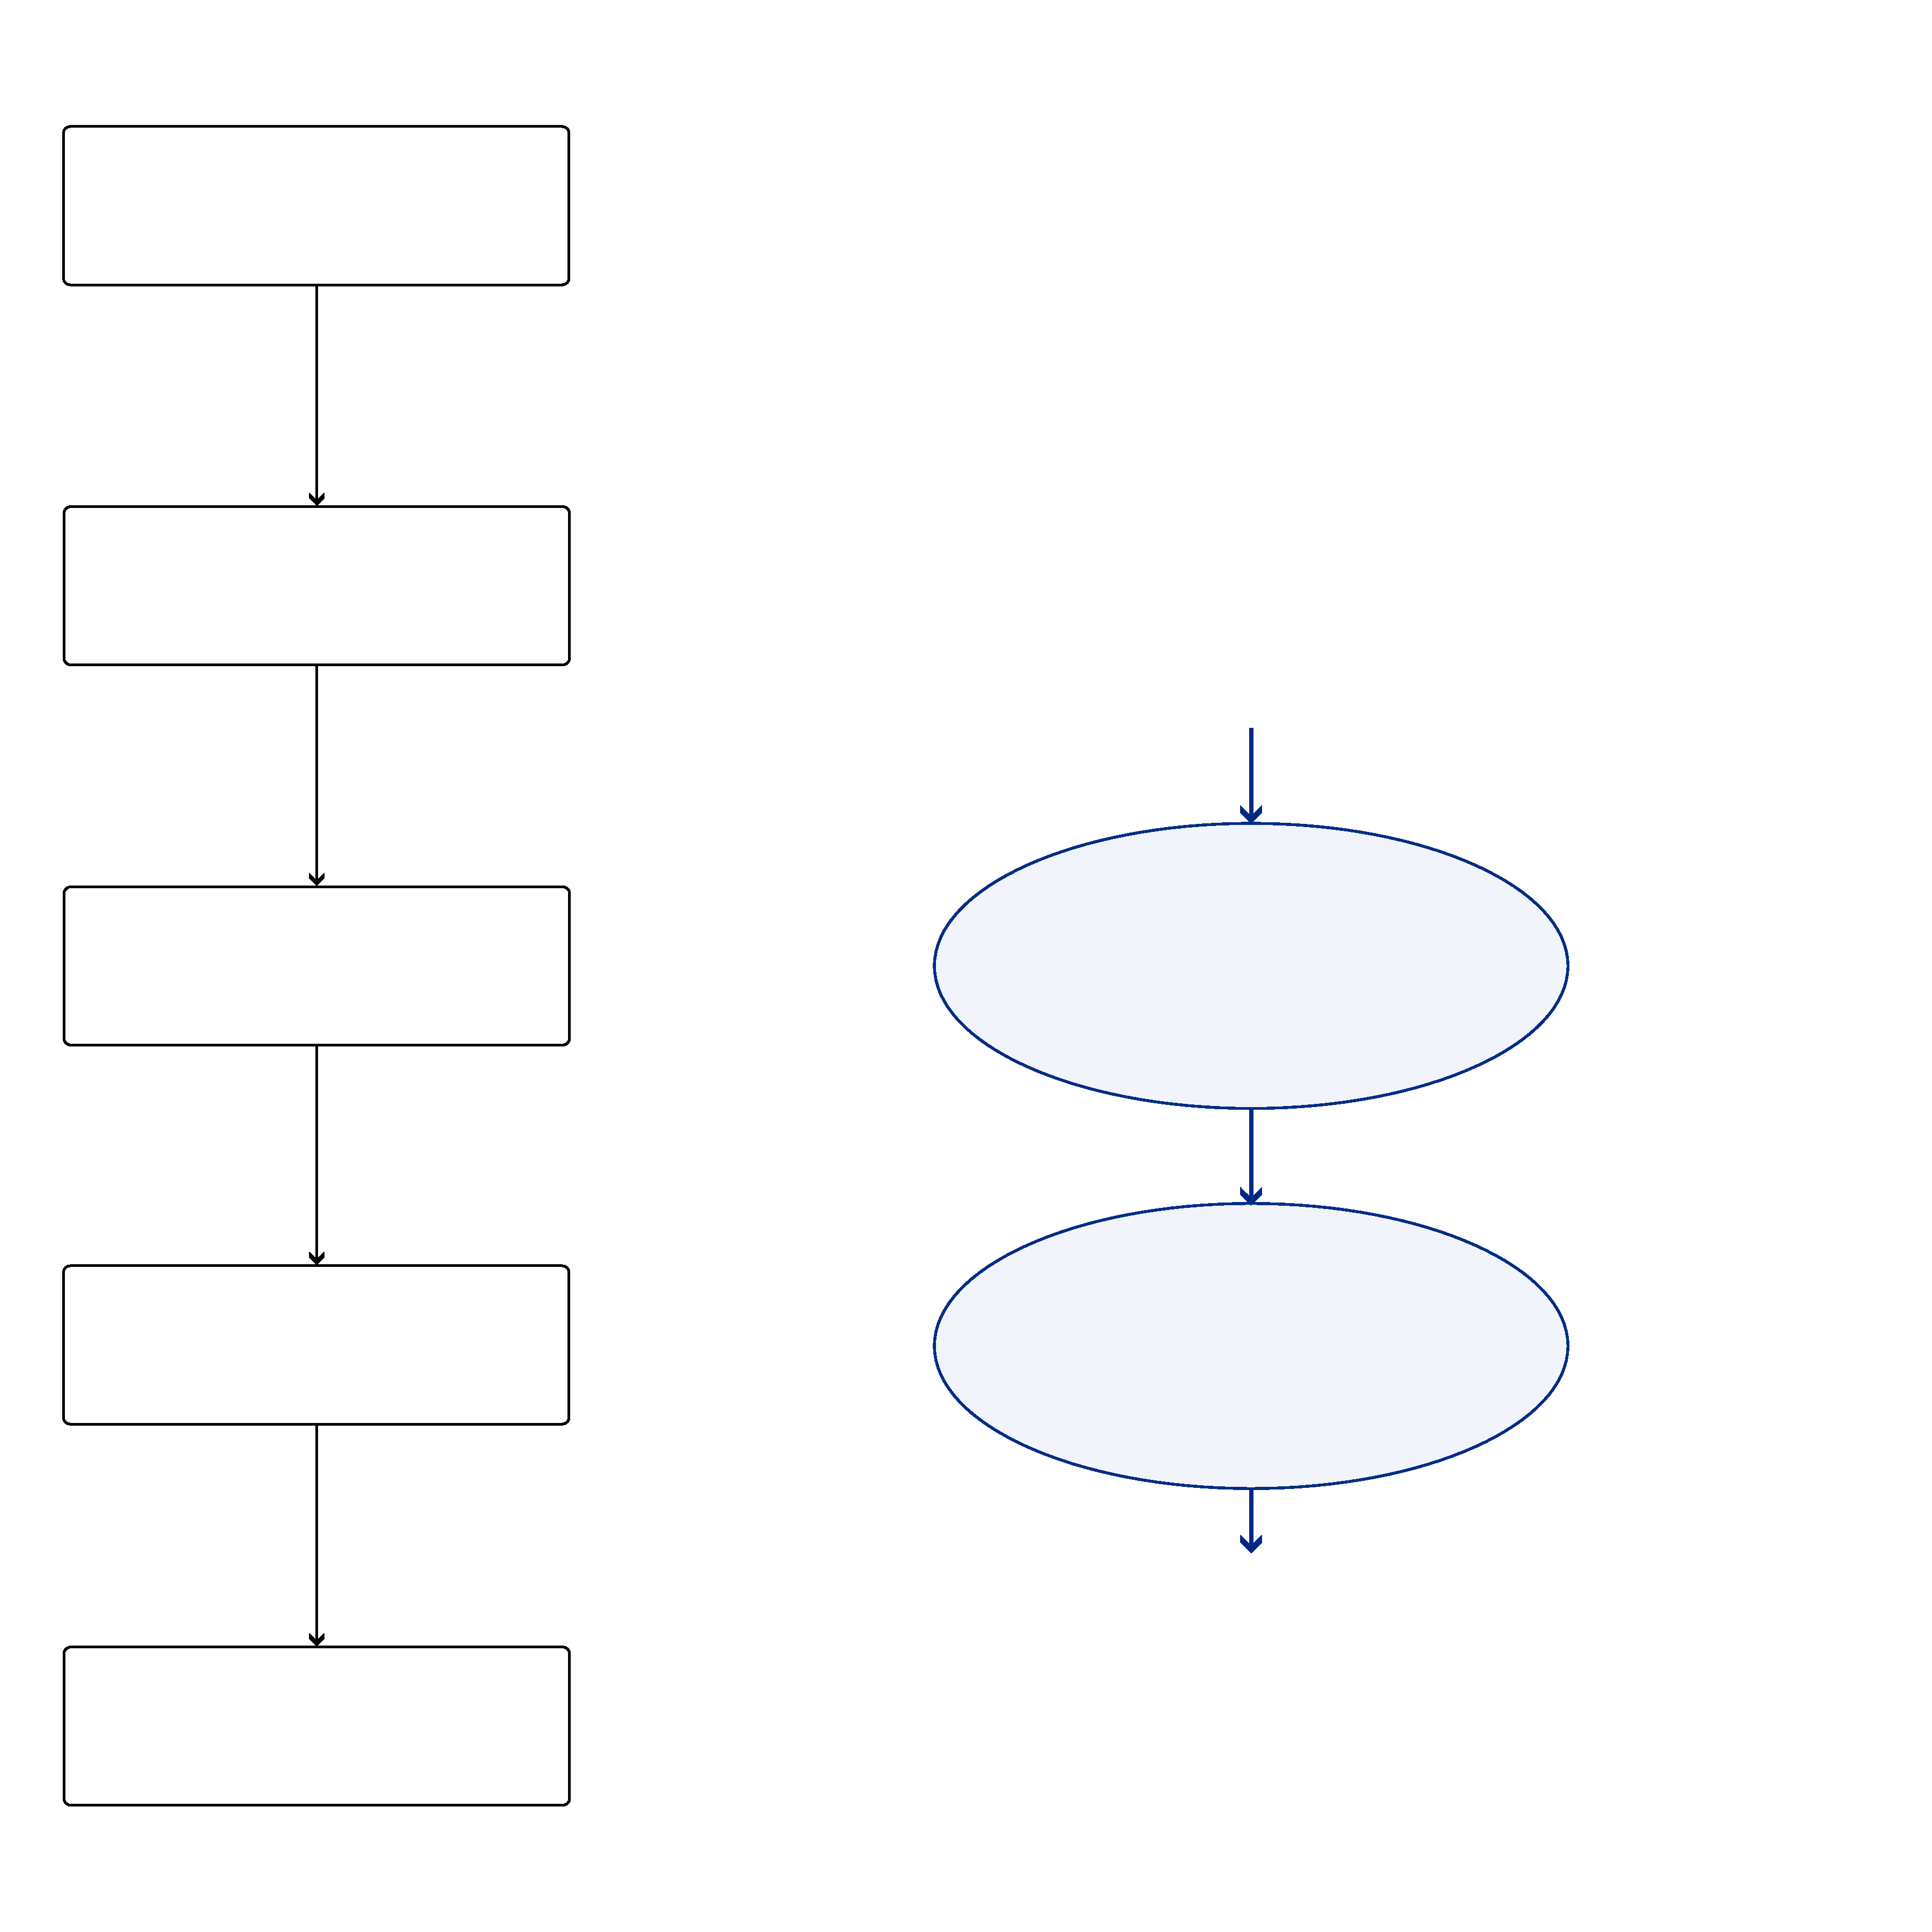
\includegraphics[width=1\linewidth]{ch4_anomalien/abbildungen/vorlage_SWIFD_schema.pdf}};
        \begin{scope}[x={(image.south east)},y={(image.north west)}]
            \node at (0.16,0.89) {\large \parbox{4cm}{\centering \textbf{Eingangssignal}:\\Zeitserie}};
            \node at (0.65,0.89) {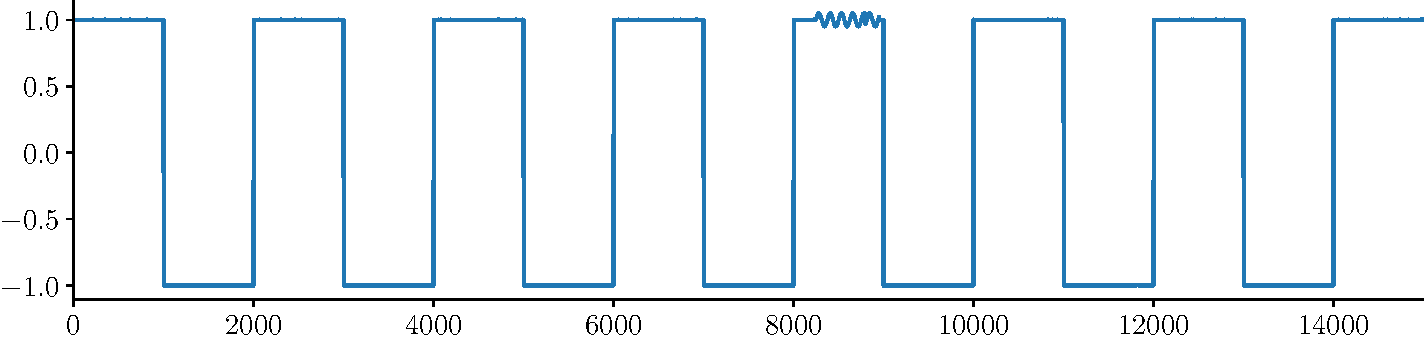
\includegraphics[width=0.68\linewidth]{ch4_anomalien/abbildungen/noisy_square_wave.pdf}};
            \node at (0.16,0.695) {\large \parbox{4cm}{\centering \textbf{1. Schritt}:\\Feature Matrix}};
            \node at (0.65,0.695) {
                    \begin{tikzpicture}
                        \node at (0,1) {$F = \begin{pmatrix} 
                            \mu_{0} & \mu_{1} & \dots & \mu_{_n-1} \\
                            \sigma_{0} & \sigma_{1} & \dots & \sigma_{_n-1} \\
                            \text{min}_{0} & \text{min}_{1} & \dots & \text{min}_{n-1} \\
                            \text{max}_{0} & \text{max}_{1} & \dots & \text{max}_{n-1} \\
                        \end{pmatrix}$};
                    \end{tikzpicture}
            };
            \node at (0.16,0.5) {\large \parbox{4cm}{\centering \textbf{2. Schritt}:\\Isolation Forest}};
            \node at (0.65,0.5) {\large \parbox{4cm}{\centering \textbf{Anomalien in Feature Matrix finden}}};
            \node at (0.16,0.305) {\large \parbox{4cm}{\centering \textbf{3. Schritt}:\\Anomalien abtragen}};
            \node at (0.65,0.305) {\large \parbox{4cm}{\centering \textbf{Für alle Fenstergrößen aufsummieren}}};
            \node at (0.16,0.11) {\large \parbox{4.2cm}{\centering \textbf{4. Schritt}:\\Dichtekarte berechnen}};
            \node at (0.65,0.11) {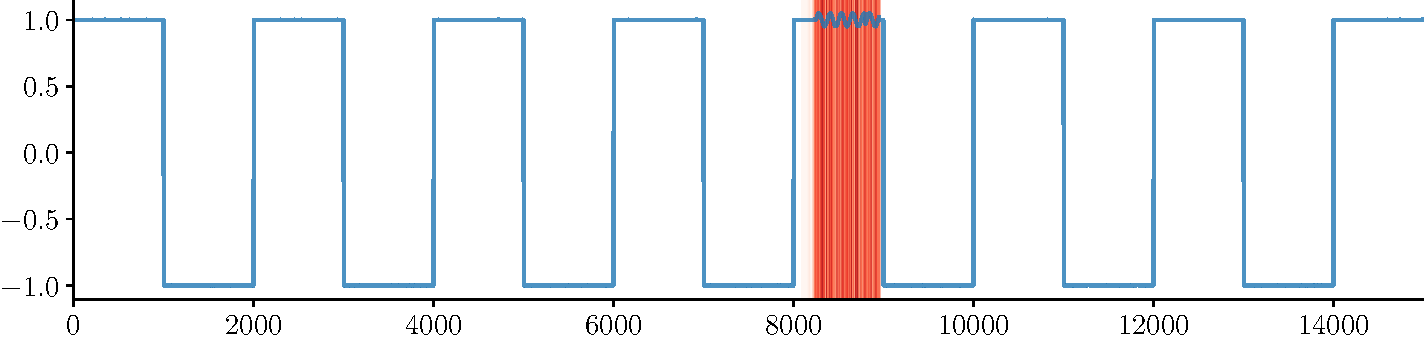
\includegraphics[width=0.68\linewidth]{ch4_anomalien/abbildungen/SWIFD_heatmap.pdf}};
        \end{scope}
    \end{tikzpicture}
    \caption{Schematischer Ablauf des SWIFD Algorithmus}
~\label{fig:swifd_schema}
\end{figure}

Der Algorithmus namens \textbf{Sliding Window Isolation Forest Density}~-~kurz \textbf{SWIFD}~-~dient der Anomalieerkennung in Zeitreihen durch die Berechnung einer
Anomaliedichtekarte mittels des Isolation Forest-Verfahrens~\cite{Liu2012}. Der schematische Ablauf ist dabei~\hyperref[fig:swifd_schema]{Abb.~\Ref*{fig:swifd_schema}}
zu entnehmen. Zunächst werden aus der Zeitreihe über gleitende Fenster statistische Merkmale
extrahiert. Hierzu wird die Zeitreihe segmentiert, wobei jedes Fenster durch Mittelwert, Standardabweichung, Minimum und Maximum beschrieben wird. Die
Fenstergröße wird aus einer vordefinierten Menge gewählt, wobei sich die Schrittweite in Abhängigkeit der Fenstergröße ergibt.

Die so gewonnenen Merkmalsvektoren werden anschließend mit dem Isolation Forest-Algorithmus verarbeitet, der auf der Grundidee von Liu et al.~\cite{Liu2012}
basiert und um die gleitenden Fenster von Ding et al.~\cite{Ding2013} weiterentwickelt wurde. Dieser konstruiert Entscheidungsbäume, in denen isolierte
Datenpunkte~–~also potenzielle Anomalien~–~mit kürzeren Pfaden identifiziert werden als
reguläre Datenpunkte. Während herkömmliche Isolation-Forest-Ansätze binäre Entscheidungen über Anomalien treffen, integriert SWIFD eine Dichtebetrachtung.
Anstatt einzelne Punkte als Anomalien zu markieren, wird für jedes Fenster ein Dichtewert berechnet, indem erkannte Anomalien aufsummiert werden.

Um lokale Schwankungen zu glätten und die visuelle Interpretierbarkeit zu verbessern, erfolgt abschließend eine Glättung der Anomaliedichte mithilfe eines
Gaußschen Filters. Dieser Ansatz kombiniert somit die Effizienz von Isolation Forest mit einer kontinuierlichen Dichteschätzung, wodurch nicht nur isolierte
Anomalien erkannt, sondern auch Bereiche mit einer erhöhten Anomaliewahrscheinlichkeit identifiziert werden können. Dies ist besonders nützlich für die
Analyse von Zeitreihen mit strukturellen Veränderungen, bei denen einzelne Punktanomalien möglicherweise nicht ausreichen, um ein klares Bild der zugrunde
liegenden Muster zu liefern.

\subsection{Mahalanobis-Distanz mit SWIFD}
Der Algorithmus \textbf{Mahalanobis-Distanz mit SWIFD}~-~kurz \textbf{MD-SWIFD}~-~wird zur Detektion von Korrelationsanomalien eingesetzt und kombiniert zwei
wesentliche Konzepte: die Mahala\-nobis-Distanz und Isolation Forest, wie er in~\hyperref[subsec:swifd]{Abs.~\Ref*{subsec:swifd}} bereits
zur Subsequenzanomaliedetektion angewandt wird. Die Weiterentwicklung um die Mahalanobis-Distanz ermöglicht die Erkennung von Anomalien in der Korrelation
in multivariaten Zeitserien~\cite{McLachlan1999}.

Als eine Erweiterung der euklidischen Distanz wird sie in multivariaten Datensätzen verwendet, um die Entfernung eines Punktes von einem Mittelwert unter
Berücksichtigung der Korrelationen zwischen den Dimensionen zu messen. Für einen Punkt $x$ in einer multivariaten Zeitserie, den Mittelwert $\mu$ und die
Kovarianzmatrix $\Sigma$, wird die Mahalanobis-Distanz $D_M$ wie folgt berechnet:

\begin{equation}
    D_M(x)\, = \sqrt{{\left( x\,-\,\mu \right)}^T\, \Sigma^{-1}\,(x\,-\,\mu)}
\label{eq:mahalanobis_dist}
\end{equation}

\begin{figure}[t!]
    \centering
    \begin{tikzpicture}
        \node[anchor=south west,inner sep=0] (image) at (0,0) {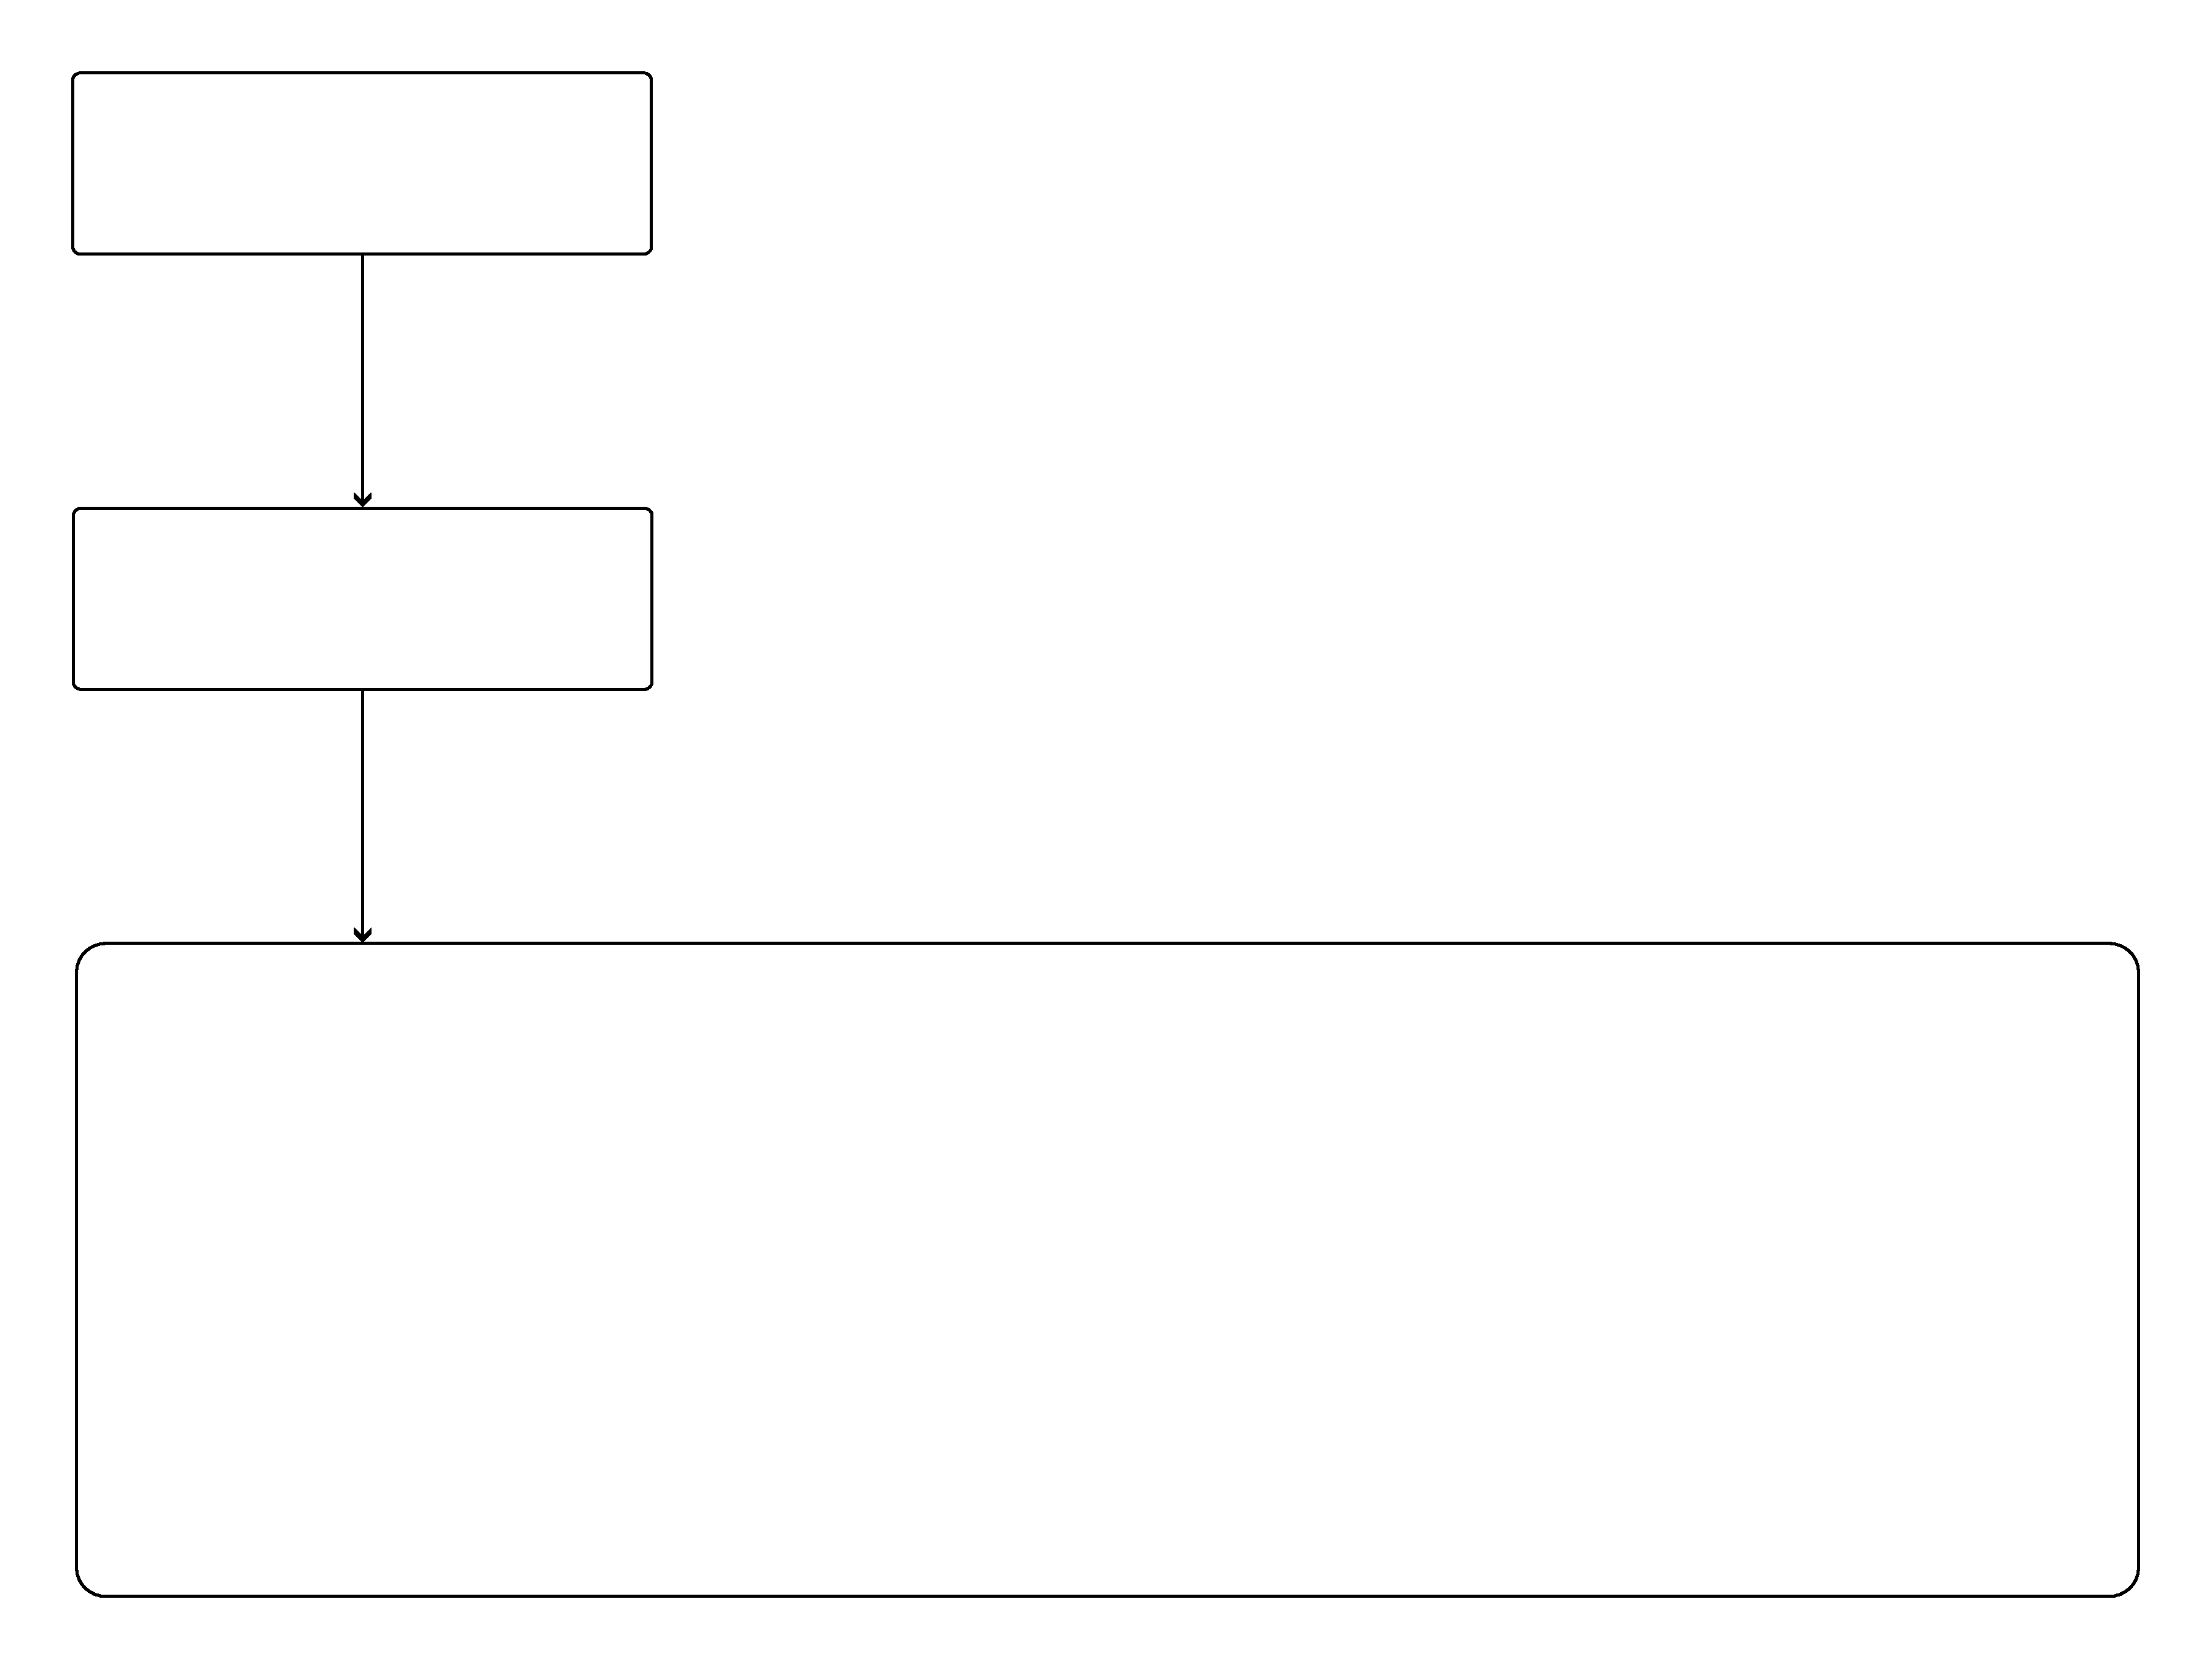
\includegraphics[width=1\linewidth]{ch4_anomalien/abbildungen/vorlage_MD-SWIFD_schema.pdf}};
        \begin{scope}[x={(image.south east)},y={(image.north west)}]
            \node at (0.16,0.9) {\large \parbox{4cm}{\centering \textbf{Eingangssignal}:\\Zeitserie}};
            \node at (0.65,0.76) {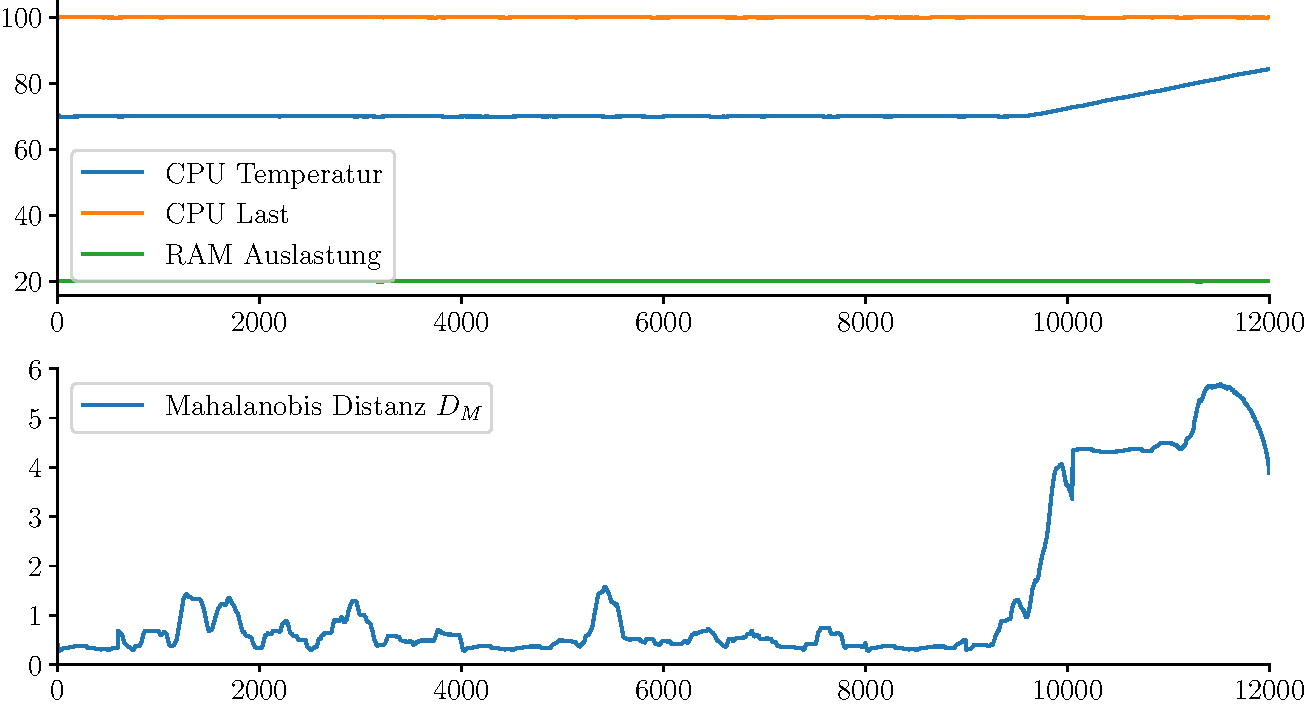
\includegraphics[width=0.68\linewidth]{ch4_anomalien/abbildungen/combined_plots.pdf}};
            \node at (0.16,0.645) {\large \parbox{4cm}{\centering \textbf{1. Schritt}:\\Mahalanobis Distanz}};
            \node at (0.5,0.39) {\large \parbox{8cm}{\centering \textbf{alle weiteren Schritte}:\\identisch zu SWIFD}};
            \node at (0.5,0.2) {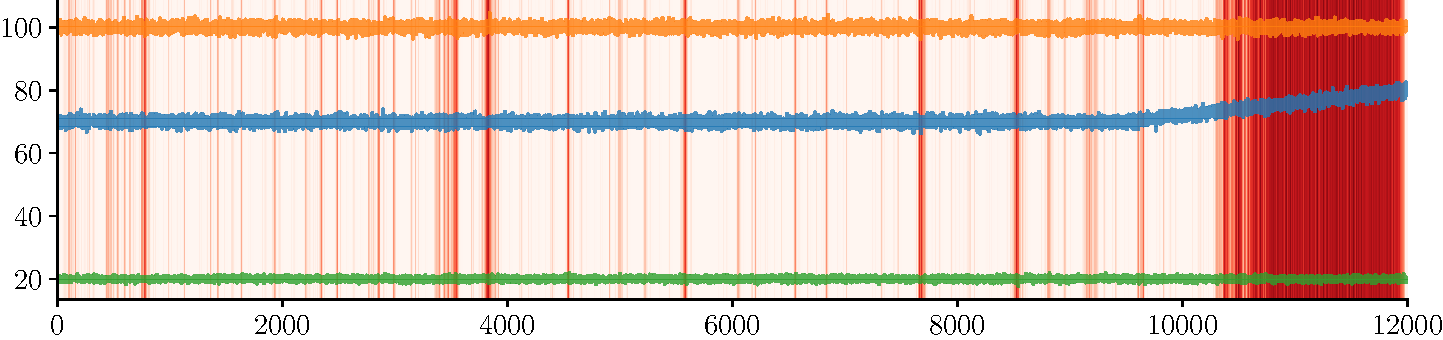
\includegraphics[width=0.9\linewidth]{ch4_anomalien/abbildungen/md_swifd_result_schema.pdf}};
        \end{scope}
    \end{tikzpicture}
    \caption{Schematischer Ablauf des MD-SWIFD Algorithmus als Erweiterung von SWIFD}
~\label{fig:md_swifd_schema}
\end{figure}

Die Mahalanobis-Distanz ist ein Maß dafür, wie stark ein Datenpunkt vom Mittelwert abweicht, wobei die Kovarianzmatrix die Streuung und die Korrelationen
zwischen den Variablen der Zeitserie berücksichtigt. In Verbindung mit SWIFD wird der \glqq zeitliche Verlauf\grqq~der Mahalanobis-Distanz~-~also die
Mahalanobis-Distanz, die zu jedem Zeitstempel der Zeitserie korrespondiert~-~als Analysesignal verwendet. In der Mahalanobis-Distanz stecken sämtliche
Informationen über das Korrelationsverhalten der Zeitserie und so können am Verlauf der Distanz Anomalien detektiert werden.

MD-SWIFD macht sich also die Funktionalität von SWIFD zu Nutze und kann so in der weiterentwickelten Version Anomalien in der Korrelation mehrerer Variablen
zuverlässig detektieren.

\subsection{Elliptic Envelope Ansatz}
Unter der Annahme, dass Daten einer multivariaten Normalverteilung folgen, wird der Elliptic Envelope verwendet, um Ausreißer in einem Datensatz zu
identifizieren. Der Algorithmus geht davon aus, dass die Mehrheit der Datenpunkte innerhalb einer elliptischen Region um den Mittelpunkt der Verteilung
liegt. Ziel des Verfahrens ist es, eine elliptische Grenze zu bestimmen, die die zentrale Datenverteilung beschreibt. Punkte, die außerhalb dieser Grenze
liegen, gelten als Ausreißer.

\begin{figure}[t!]
    \centering
        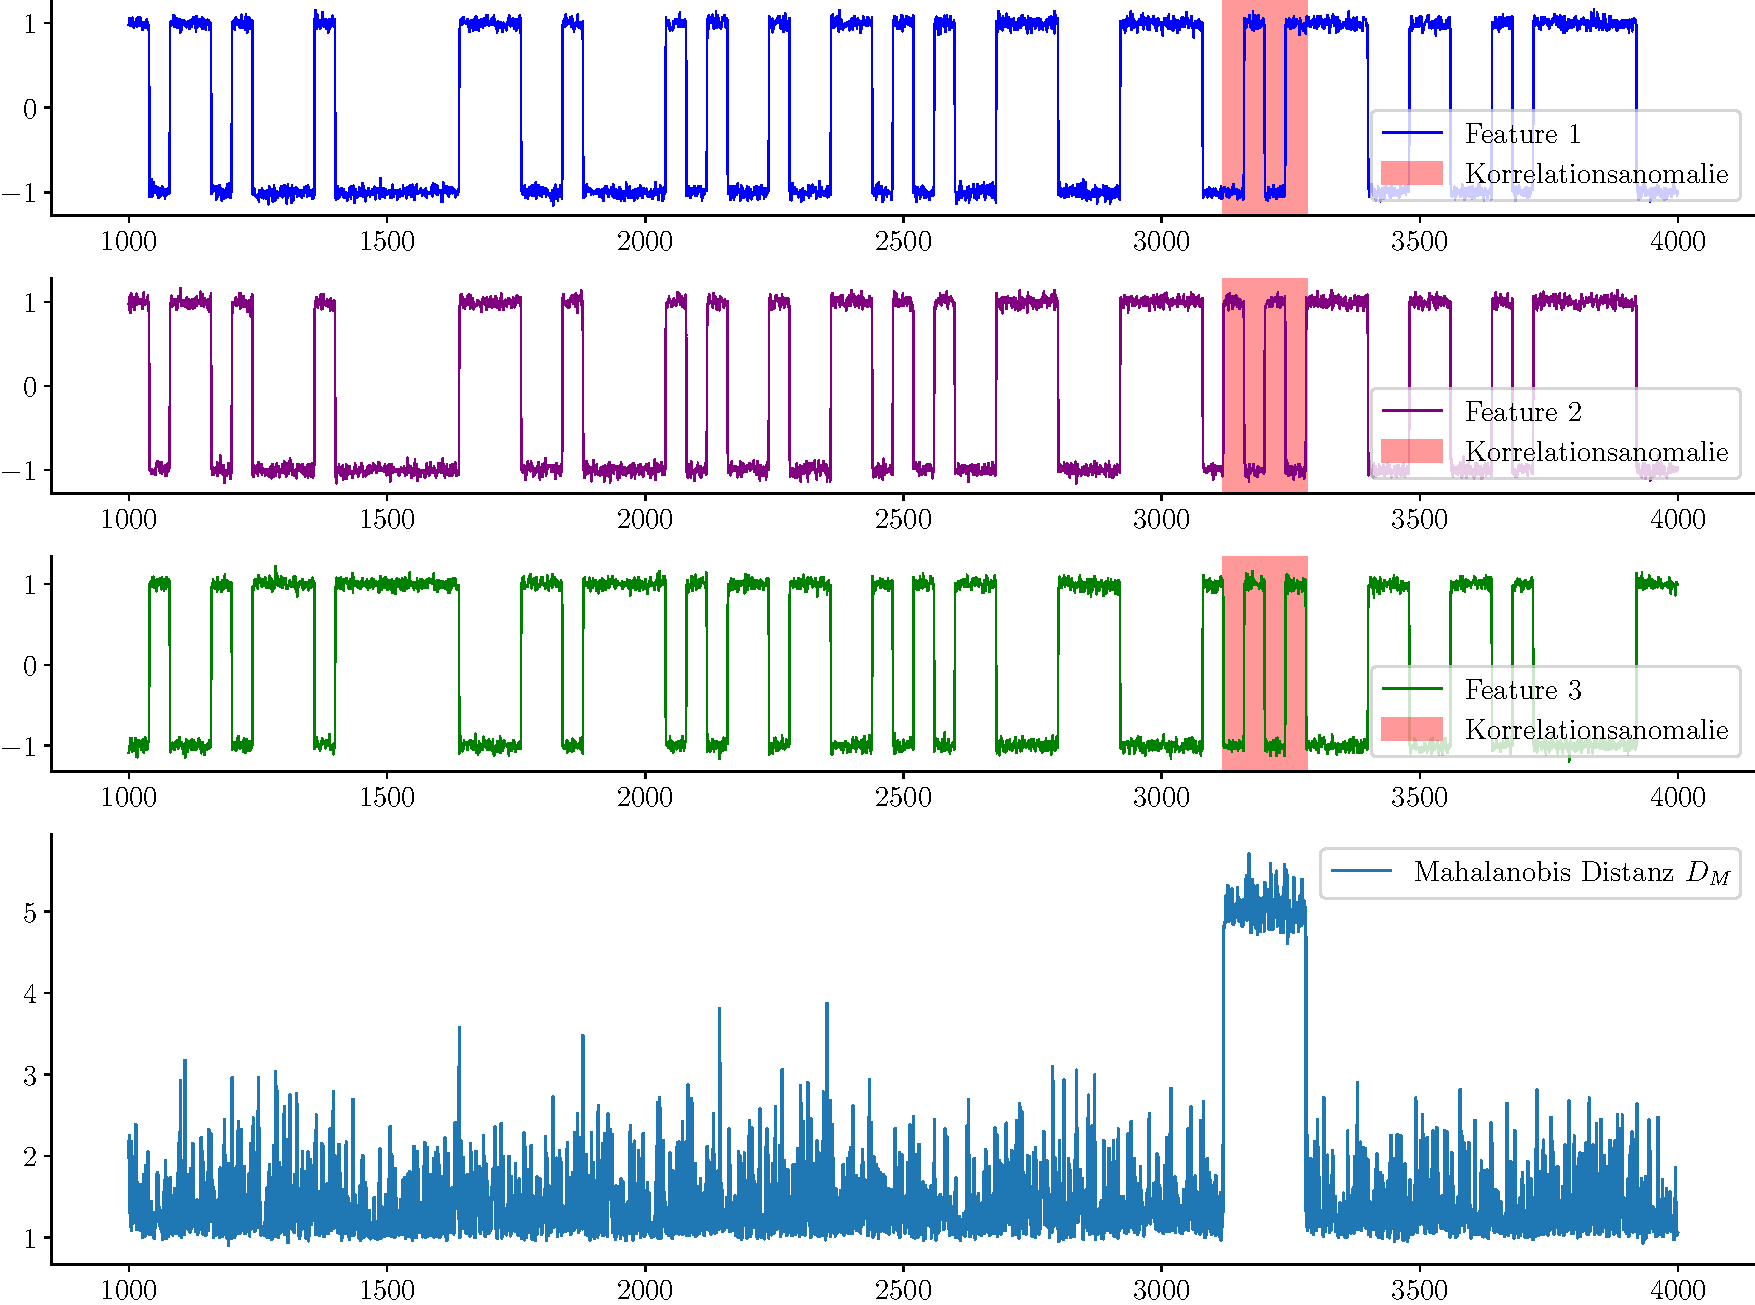
\includegraphics[width=1\linewidth]{ch4_anomalien/abbildungen/EE_mahalanobis.pdf}
    \caption{Ausschnitt aus dreidimensionaler Zeitreihe mit entsprechender Mahalanobis Distanz $D_M$. Anhand von $D_M$ können Korrelationsanomalien
        durch Setzen eines Schwellwerts erkannt werden, wenn die Distanz oberhalb dieser Schwelle liegt.}
\label{fig:EE_mahalanobis}
\end{figure}

Die Funktionsweise des Elliptic Envelope basiert auf der Schätzung der Kovarianzmatrix der Daten und der Bestimmung einer Ellipse, die diese am besten
beschreibt. Mithilfe des Maximum-Likelihood-Verfahrens wird die multivariate Normalverteilung ermittelt, die die größten Anteile der Daten umfasst. Die
Hauptachsen dieser Ellipse werden durch die Eigenwerte und Eigenvektoren der Kovarianzmatrix bestimmt. Um Ausreißer zu erkennen, wird eine
Mahalanobis-Distanz berechnet, und Datenpunkte, die eine zu hohe Distanz aufweisen, werden als Anomalien identifiziert~\cite{Ashrafuzzaman2020}.

Der Elliptic Envelope wird häufig in Bereichen eingesetzt, in denen die Annahme einer Normalverteilung zutrifft, wie beispielsweise in der Analyse von
verdächtigen Netzwerkaktivitäten~\cite{Ashrafuzzaman2020}. Besonders nützlich ist der Algorithmus bei hochdimensionalen Daten, in denen
einfache univariate Verfahren an ihre Grenzen stoßen. Da der Elliptic Envelope Korrelationen zwischen den Variablen berücksichtigt, kann er auch
komplexere Datenstrukturen als univariate Methoden erfassen.

\begin{figure}[t!]
    \centering
        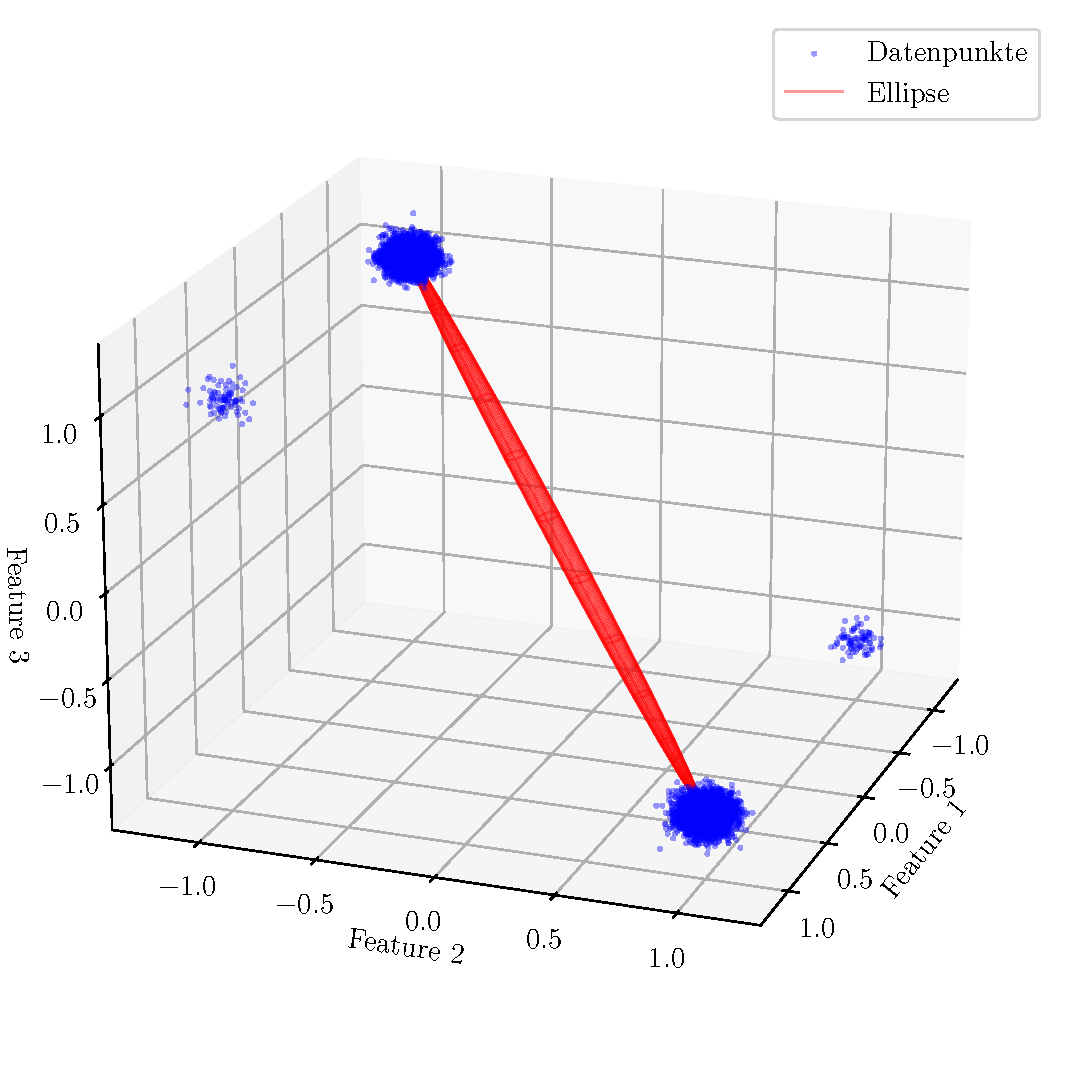
\includegraphics[width=1\linewidth]{ch4_anomalien/abbildungen/EE_ellipse.pdf}
    \caption{Ellipsoid auf Basis der Kovarianz der drei Kanäle}
    \label{fig:ee_ellipse}
\end{figure}

\section{Semi-Supervised Learning Algorithmen}
Eine weitere Möglichkeit der Anomaliedetektion ist die mit Algorithmen der Klasse \textbf{Semi-Supervised Learning}. Algorithmen dieser Klasse benötigen
Trainingsdaten, die dem Normal entsprechen und sind daher zu Beginn der Implementierung zunächst unpraktischer als die der Klasse Unsupervised Learning.
Der Grund dafür ist, dass erst eine erhebliche Menge an Training durchgeführt werden muss, optimalerweise mit Daten, die den gesamten normalen Betriebsbereich
abdecken können~\cite[S.~2-4]{Chapelle2010}~\cite{Schmidl2022}. Dementsprechend werden Datenpunkte- oder sequenzen, die nicht dem Normal angehören oder
als solches identifiziert werden können, als Anomalie gekennzeichnet.

Das Sammeln von großen Datensätzen ist kein Problem. Das SSP X1 System nimmt beispielsweise im Sekundentakt Daten auf und so entstehen schnell große
Datensätze bzw.~Zeitserien. Die Problematik liegt vielmehr darin, dass die Daten mit einem Label versehen werden müssen, zumindest implizit. Es muss
sichergestellt sein, dass die gesamte vorliegende Zeitserie einem normalen Betriebszustand entspricht~\cite[S.~10~ff]{Chapelle2010}.

\subsection{LSTM-Autoencoder}
Einer in seiner Funktionalität interessanter Algorithmus ist der LSTM-Autoencoder (LSTM-AE). LSTM steht für Long-Short Term Memory, ist eine Erweiterung der
Recurrent Neural Networks und erlaubt es, auf ein Langzeitgedächtnis zurückzugreifen und kommt gänzlich ohne Parametrisierung aus~\cite{Hochreiter1997}.
Ein Autoencoder ist ein Algorithmus, der auf Basis der Rekonstruktion von Sequenzen Anomalien detektiert und gehört demnach zur Kategorie der
Subsequenzanomaliedetektion~\hyperref[tab:algorithmen]{(vgl.~Tab.~\Ref*{tab:algorithmen})}.

Die Einordnung in die Klasse der Rekonstruktionsalgorithmen erfolgt nach Schmidl et al.~\cite{Schmidl2022} und beschreibt Rekonstruktionsalgorithmen
als solche, die Subsequenzen in eine niederdimensionalere Do\-mäne enkodieren, von wo sie wieder dekodiert bzw.~rekonstruiert werden. Ein zu analysierender
Datensatz wird also in Subsequenzen unterteilt und diese werden enkodiert. Mithilfe der Trainingsdaten werden die enkodierten Sequenzen rekonstruiert,
wobei Abweichungen des Originals zur rekonstruierten Sequenz als Anomalie gelten dürfen, da sie mit den Trainingsdaten nicht übereinstimmen.

Die Kombination der beiden Prinzipien zum LSTM-AE erlaubt die Enkodierung der Subsequenzen unter Beibehalt langzeitiger Abhängigkeiten und Korrelationen
und erweist sich so als sehr geeignet für große multivariate Zeitserien mit unterschiedlichen Abhängigkeiten und Korrelationen, wie sie in den Systemen
der SSP X1 vorkommen~\cite{Wei2022}.

Der Algorithmus wird im nächsten Kapitel denselben Tests unterzogen wie seine Unsupervised Learning Pendants. Schlussendlich ist auch eine
Implementierung von LSTM-AE zur Anomaliedetektion im Kontext der SSP X1 und verwandter Systeme nicht auszuschließen.

\section{Übersicht über alle ausgewählten Algorithmen}

Abschließend folgt eine kurze Auflistung aller genannten Algorithmen mit stichwortartiger Kategorisierung nach Detektionsklasse, -prinzip sowie die Quelle der
Implementierung. Unter dem Stichwort \textit{Eigene Implementierung} verbergen sich auch Komponenten, die aus Python Bibliotheken angewandt wurde, wie der
Algorithmus zu \textbf{Isolation Forest}~\cite{scikit-learn} oder die Implementierung des \textbf{LSTM}~\cite{pytorch}, die zur gewollten Funktionalität
zusammengeführt und erweitert wurden. Im nächsten Kapitel erfolgt die Erprobung, Gegenüberstellung und Evaluierung sämtlicher Algorithmen derselben
Detektionsklasse.

\begin{table}[h]
    \renewcommand{\arraystretch}{1.75}
    \begin{tabular}{c||c|c|c}
\textbf{Algorithmus}                        & \textbf{Detektionsklasse}     & \textbf{Detektionsprinzip}   & \textbf{Quelle}               \\
\hline
\textbf{HBOS}                               & Punktanomalien        & Histogramm          & PyOD (Open Source)~\cite{zhao2019pyod}     \\
\hline
\multirow{2}{*}{\textbf{Sliding Window}}    & \multirow{2}{*}{Punktanomalien}        & \multirow{2}{*}{Z-Score} & \multirow{2}{*}{Eigene Implementierung} \\
\textbf{Z-Score} & & & \\
\hline
\textbf{GrammarViz 2.0}                     & Subsequenzanomalien   & Grammatik           & Open Source~\cite{senin-gv2}           \\
\hline
\textbf{SWIFD}                              & Subsequenzanomalien   & Isolation Tree      & Eigene Implementierung     \\
\hline
\multirow{2}{*}{\textbf{MD-SWIFD}}          & \multirow{2}{*}{Korrelationsanomalien} & \multirow{2}{*}{Mahalanobis Distanz} & \multirow{2}{*}{Eigene Implementierung} \\
 & & und Isolation Tree & \\
\hline
\multirow{2}{*}{\textbf{Elliptic Envelope}} & \multirow{2}{*}{Korrelationsanomalien} & \multirow{2}{*}{Kovarianzmatrix und} & \multirow{2}{*}{sklearn (Open Source)~\cite{scikit-learn}} \\
 & & Mahalanobis Distanz & \\
\hline\hline
\multirow{2}{*}{\textbf{LSTM-AE}}           & \multirow{2}{*}{Subsequenzanomalien}   & \multirow{2}{*}{Rekonstruktion und} & \multirow{2}{*}{Eigene Implementierung} \\
 & & Neuronale Netze &
\end{tabular}
    \caption{\centeringÜbersicht über die verwendeten Algorithmen nach Kategorisierung in Detektionsklasse, Detektionsprinzip und Ursprung}
~\label{tab:algorithmen}
\end{table}

% Literaturverzeichnis hinzufügen und verlinken
\addcontentsline{toc}{chapter}{Literaturverzeichnis}
\printbibliography[]

\end{document}
